\documentclass[11pt,a4paper]{article}
\usepackage[T1]{fontenc}
\usepackage[utf8]{inputenc}
\usepackage{newtxtext,newtxmath}
\usepackage[margin=25mm,headheight=15pt]{geometry}
\usepackage{microtype,graphicx,xcolor,amsmath}
\usepackage{booktabs,tabularx,longtable,array,float}
\usepackage{algorithm,algpseudocode}
\usepackage{listings}
\usepackage{tikz,pgfplots}
\usetikzlibrary{arrows.meta,positioning,calc,fit,backgrounds}
\pgfplotsset{compat=1.18}
\usepackage[numbers,sort&compress]{natbib}
\usepackage{enumitem,fancyhdr}
\usepackage[colorlinks=true,linkcolor=Ink,citecolor=Teal,urlcolor=Teal,breaklinks=true]{hyperref}
\usepackage[nameinlink,noabbrev]{cleveref}
\makeatletter
\providecommand{\theHALG@line}{}
\renewcommand{\theHALG@line}{\thealgorithm.\arabic{ALG@line}}
\makeatother
% Shared vocabulary and editable diagram styles for paper and Beamer.
\definecolor{Ink}{HTML}{17324D}
\definecolor{Teal}{HTML}{087F8C}
\definecolor{Amber}{HTML}{A8670A}
\definecolor{Pale}{HTML}{EEF5F7}
\definecolor{Muted}{HTML}{526374}
\newcommand{\revision}{498dea0}
\newcommand{\snapshotdate}{25 November 2026}
\newcommand{\SAT}{\operatorname{SAT}}
\newcommand{\UNSAT}{\operatorname{UNSAT}}
\newcommand{\True}{\mathsf{true}}
\newcommand{\False}{\mathsf{false}}
\newcommand{\code}[1]{\texttt{\detokenize{#1}}}
\newcommand{\example}[1]{\paragraph{\textcolor{Teal}{#1}}}
% Source pointers remain in the editable text and evidence index.
\newcommand{\source}[1]{\par}
\tikzset{stage/.style={draw=Ink,thick,rounded corners=2pt,align=center,fill=Pale,minimum height=1.05cm,text width=2.65cm,font=\small},
  flow/.style={-{Stealth[length=2mm]},thick,draw=Teal},
  annotation/.style={font=\scriptsize,align=center,text=Muted}}

% Permanent links to the exact example texts preserved in the source snapshot.
\newcommand{\orderurl}{https://github.com/unibuc-cs/spelcheck/blob/498dea06df250964013b2abb2b06c94d341b223b/specs/order/requirements.md}
\newcommand{\authbaseurl}{https://github.com/unibuc-cs/spelcheck/blob/498dea06df250964013b2abb2b06c94d341b223b/specs/auth_change/openspec/specs/auth/spec.md}
\newcommand{\authchangeurl}{https://github.com/unibuc-cs/spelcheck/blob/498dea06df250964013b2abb2b06c94d341b223b/specs/auth_change/openspec/changes/admin-never-locked/specs/auth/spec.md}
\newcommand{\authfullurl}{https://github.com/unibuc-cs/spelcheck/blob/498dea06df250964013b2abb2b06c94d341b223b/specs/auth_openspec/spec.md}
\newcommand{\deletionurl}{https://github.com/unibuc-cs/spelcheck/blob/498dea06df250964013b2abb2b06c94d341b223b/specs/delete_property/requirements.md}

\lstset{basicstyle=\ttfamily\small,columns=fullflexible,keepspaces=true,
  showstringspaces=false,breaklines=true,frame=single,
  rulecolor=\color{Teal!35},backgroundcolor=\color{Pale},
  aboveskip=6pt,belowskip=6pt,xleftmargin=4pt,xrightmargin=4pt}
\setlength{\parindent}{0pt}
\setlength{\parskip}{5pt plus 1pt}
\setlength{\emergencystretch}{2em}
\setlist[itemize]{leftmargin=*,itemsep=2pt,topsep=3pt}
\setlist[enumerate]{leftmargin=*,itemsep=2pt,topsep=3pt}
\renewcommand{\arraystretch}{1.15}
\pagestyle{fancy}\fancyhf{}
\fancyhead[L]{\small\color{Muted}speccheck / technical progress report}
\fancyfoot[C]{\small\thepage}
\renewcommand{\headrulewidth}{0.3pt}
\hypersetup{pdftitle={speccheck: Checking requirements with language models and Z3},pdfsubject={Technical progress report, revision 498dea0}}
\setcounter{tocdepth}{2}
\begin{document}
\hypersetup{pageanchor=false}
\begin{titlepage}
\vspace*{15mm}
{\sffamily\color{Teal}\large TECHNICAL PROGRESS REPORT\par}
\vspace{8mm}
{\sffamily\bfseries\color{Ink}\fontsize{30}{35}\selectfont speccheck\par}
\vspace{4mm}
{\sffamily\color{Ink}\LARGE Checking requirements with\\language models and Z3\par}
\vspace{8mm}
{\large Method, evaluation and limitations\par}
\vspace{10mm}
\hrule
\vspace{5mm}
\begin{abstract}
Natural-language requirements can be individually clear yet impose incompatible obligations when read together. This report studies a prototype that translates requirements with a language model, checks the resulting formulas with Z3, and returns review questions with witnesses and explicit assumptions. The method tests competing translations, asks about relations between separately named outcomes, and checks proposed OpenSpec changes against existing requirements.

The experiments examine conflict detection, ambiguity, change analysis and scale. In E18, outcome-pair questions increased planted conflict detections from 27/36 to 34/36 across repeated runs, while clean runs with a conflict alarm increased from 0/18 to 3/18. Second-reader experiments found more planted ambiguities and raised more questions about clean specifications. E19 tested removal handling and found 35/36 planted gaps. In E20, reusing a saved base model reduced mean formalization requests per change from 68 to 9, after an initial mean 61 requests per base; conflict detections fell from 54/54 to 50/54. Full formalization remains the default. The scale exercises reached 100 requirements, with input and representation limits still apparent.

These results support further study of assisted requirements review. They do not establish faithful translation, production defect rates or human review savings. The evidence comes mainly from project-authored examples, and the snapshot representation can confuse successive states or separate objects. Reuse currently follows scenario edits and can miss a change confined to a requirement sentence. The next work is independent evaluation, broader edit coverage and better vocabulary selection.
\end{abstract}

\vfill
{\color{Muted}\snapshotdate\quad\textbullet\quad Version \code{498dea0}\par}
\end{titlepage}
\pagenumbering{roman}
\hypersetup{pageanchor=true}
{\small\setlength{\parskip}{0pt}\tableofcontents}
\clearpage
\pagenumbering{arabic}
\section{Problem and running example}\label{sec:intro}\label{sec:problem}

Suppose an authentication specification says to lock an account after five failed attempts. A proposed change says that administrators must never be locked out. Both sentences are easy to read. Together, they give the implementation an impossible job when an administrator reaches five failed attempts.

We want a requirements checker to bring that decision back to the author: identify the conflicting rules, show a situation in which they clash, and explain what needs to be resolved. A general warning that the specification may be inconsistent leaves too much work to the reviewer. The harder cases arise when the obligations use different words, when a condition admits several readings, or when a proposed change conflicts with a requirement elsewhere.

The project is a small reconstruction and investigation of the formal-analysis idea described in Kiro's requirements-analysis article~\citep{kiro2026}. It is not Kiro's implementation, and these experiments are not a head-to-head product comparison. The approach uses a language model to translate requirements, Z3~\citep{z3} to check the formulas, and a language model to explain the findings. Formal checking can establish a result about the supplied formulas; it cannot establish that the translation preserves the author's intent.

The project provides a working pipeline with saved translations, solver witnesses and explicit assumptions; mechanisms for challenging translations and connecting separately named outcomes; and change checking that retains removal evidence and optionally reuses a saved base model. This report connects those procedures to experiments showing their gains, costs and remaining limits.

The evaluation uses project-authored specifications and planted defects. It supports conclusions about these examples and comparisons, rather than production defect rates or measured savings in human review time. Authentication provides a common example for the four finding types and the OpenSpec change workflow. Order processing supplies a second worked example for the detailed solver procedures; property deletion illustrates uncertain relations between outcomes. Detailed pseudocode, full models and the saved order walkthrough are in the appendices.
\source{speccheck/cli.py; speccheck/formalize.py; speccheck/change.py}

\subsection{The authentication example}

The running example starts with an \href{\authbaseurl}{authentication specification in OpenSpec} and a \href{\authchangeurl}{proposed administrator exception}. The baseline has two requirements, Login and Account Lockout, containing four scenarios. The change adds a fifth scenario. Both files are available on GitHub for readers who want the complete wording and project layout.

We describe one snapshot, not a sequence of login attempts. Let $p$ mean a password is submitted, $v$ that it is correct, $g$ that access is granted, $d$ that access is denied, $n$ the failed-attempt count, $\ell$ that the account is locked, and $h$ that it belongs to an administrator. The Boolean symbols describe that snapshot; $n$ is an integer. Table~\ref{tab:auth-baseline} gives the selected formulas from the saved combined model. The four baseline formulas are projected from that model; they are not a separate formalization of the baseline.

\begin{table}[H]
\centering
\begin{tabularx}{\linewidth}{@{}lXl@{}}
\toprule
Rule & Scenario and required response & Selected formula \\
\midrule
R1 & Valid credentials: grant access for a correct submitted password. & $(p\land v)\Rightarrow g$ \\
R2 & Invalid credentials: deny access for an incorrect submitted password. & $(p\land\neg v)\Rightarrow d$ \\
R3 & Lockout threshold: lock when failed attempts reach five. & $(n=5)\Rightarrow\ell$ \\
R4 & Locked account: deny access when a password is submitted for a locked account. & $(p\land\ell)\Rightarrow d$ \\
\midrule
R5 & Proposed addition: never lock an administrator's account. & $h\Rightarrow\neg\ell$ \\
\bottomrule
\end{tabularx}
\caption{Authentication baseline R1--R4 and proposed addition R5. R1--R2 belong to Login; R3--R4 to Account Lockout. The exactly-five reading of R3 is itself open to review.}\label{tab:auth-baseline}
\end{table}

We distinguish three versions: $P_0=\{R1,R2,R3,R4\}$ is the baseline projection; $P_+=P_0\cup\{R5\}$ is the actual saved administrator change; and $P_-=P_0\setminus\{R2\}$ is a separate, constructed removal used below. The removal is not part of the administrator change. Rule labels are local to each example. We do not assume that the baseline is defect-free: the saved findings also contain an older R1/R4 conflict under an assumed grant/deny exclusion.
\source{specs/auth_change/openspec/specs/auth/spec.md; specs/auth_change/openspec/changes/admin-never-locked/specs/auth/spec.md; specs/auth_change/formal.json; specs/auth_change/findings.json}

\subsection{Four kinds of findings}

An encoded rule has a condition $a_i$ and an obligation $c_i$: $\phi_i=a_i\Rightarrow c_i$. Write $\Phi_P$ for the conjunction of all implications in version $P$. A result $\SAT(F)$ means that some assignment satisfies $F$; $\UNSAT(F)$ means that none does. These definitions let us state each finding and its example together. The following queries use the rules alone; later sections explain assumptions, search bounds and solver timeouts.

\begin{table}[H]
\centering
\begin{tabularx}{\linewidth}{@{}lXX@{}}
\toprule
Finding & What it establishes or asks & Authentication example \\
\midrule
Conflict & A feasible triggering situation has incompatible obligations. & In $P_+$, five failed attempts require an administrator to be both locked and unlocked. \\
Gap & An examined situation has no applicable conditional rule. & In constructed $P_-$, an incorrect password can be submitted with no remaining response. \\
Ambiguity & Competing readings or an unusable translation need interpretation review. & Does ``reaches five'' mean exactly five or at least five? \\
Scenario & The rules allow or rule out a situation the author should confirm. & $P_0$ permits access without submission; $P_+$ rules out a submitted password for a locked administrator. \\
\bottomrule
\end{tabularx}
\caption{Four review questions within one example. A gap or surprising scenario is not automatically a defect.}
\end{table}

\textbf{Conflict.} For a triggering situation $T$, the test requires $\SAT(T)$ and $\UNSAT(T\land\Phi_P)$. A situation forbidden by one rule alone is treated as a ruled-out scenario instead. In the saved addition, take $T=(n=5)\land h$. The situation is feasible, but R3 requires $\ell$ and R5 requires $\neg\ell$. Both obligations cannot be met. This clash occurs under either the exactly-five or the five-or-more reading of R3.

\textbf{Gap.} Let $C_P$ be the rules with non-tautological conditions and let $E$ fix the event context being examined. A gap satisfies $E\land\bigwedge_{i\in C_P}\neg a_i$. For the constructed removal $P_-$, set $p=\True$, $v=\ell=\False$ and $n=0$. A password is submitted, but R1, R3 and R4 are all inactive. The removed R2 used to require denial in this situation. This is missing conditional coverage; it does not claim that every business situation has been explored.

\textbf{Ambiguity.} Two readings $\phi$ and $\psi$ can be distinguished when $\SAT(\phi\mathbin{\oplus}\psi)$, where $\oplus$ is exclusive OR. For R3, $(n=5)\Rightarrow\ell$ and $(n\ge5)\Rightarrow\ell$ differ at $n=6,\ell=\False$. That snapshot obeys the first reading and violates the second. The saved interpretation probe asks about precisely this difference. A distinguishing assignment makes the question concrete; it does not establish which reading the author intended. The ambiguity procedure also considers translation agreement and whether a usable reading was obtained.

\textbf{Scenario.} An allowed consequence is witnessed by $\SAT(\Phi_P\land\neg a_i\land c_i)$: an obligation is met even though its condition is false. In $P_0$, the illustrative snapshot $p=v=\ell=d=\False$, $n=0$, $g=\True$ satisfies every rule. R1 says when to grant access, not that access is granted only then. The ruled-out search instead finds feasible combined conditions that one rule forbids on its own. In $P_+$, R4 and R5 can have the joint condition $T=p\land\ell\land h$, but $T\land\neg\ell$ is impossible because of R5. This is a consequence of the administrator policy to confirm, rather than a clash between two obligations. These scenario assignments are illustrative, not quotations from a saved report.

\subsection{Further worked examples}

\textbf{Order processing.} The detailed solver sections use a second worked example: accept a submission, decide whether stock is available, and handle cancellation. Table~\ref{tab:order} abbreviates the \href{\orderurl}{complete EARS requirements on GitHub}. Its R1--R5 labels refer to the order source rules and are separate from the authentication labels above. The full wording and saved solver identifiers remain available for inspection.

\begin{table}[H]
\centering
\begin{tabularx}{\linewidth}{@{}lXX@{}}
\toprule
Rule & When it applies & What it demands \\
\midrule
R1 & An order is submitted and stock is available & Fulfill the order. \\
R2 & An order is submitted and stock is unavailable & Put the order on backorder. \\
R3 & Always & Do not put an order on backorder. \\
R4 & An order is canceled & Refund its payments. \\
R5 & An order is in a canceled-and-refunded state & Do not fulfill it. \\
\bottomrule
\end{tabularx}
\caption{The five order requirements, with stable rule labels. The source uses EARS wording; this is not an OpenSpec change file.}\label{tab:order}
\end{table}
\source{specs/order/requirements.md}

Take the situation ``submitted, no stock.'' R2 requires backordering and R3 forbids it. The question for the author is whether to allow backorders, remove that branch of R2, or change the conditions under which one of the rules applies. The checker can identify the problem. It cannot decide which business policy is intended.

There is another clash in the example: if an order is submitted with stock while it is already canceled and refunded, R1 requires fulfillment and R5 forbids it. Whether that combination describes a meaningful moment in the real system is a separate question. That separation will become important when we discuss assumptions and time.

\textbf{Delete versus retain.} In the \href{\deletionurl}{property-deletion requirements}, D2 says to remove a property record after deletion is confirmed; D4 calls for soft deletion that retains the record for audit while hiding it from the interface. If the model invents separate symbols for ``removed'' and ``retained,'' Z3 does not know that the author might regard them as opposites. That is the example for facts, links, and outcome-pair probes. We do not assume in advance that removal means physical erasure: deciding that interpretation is precisely the difficulty.

These cases come from the project; the abbreviated symbols and constructed sample counts used to explain algorithms are illustrative.
\source{specs/delete_property/requirements.md; specs/order/requirements.md}


\subsection{Research questions}

The central question is whether this combination can produce well-supported review questions while making its translation uncertainty visible. We examine four parts of that question:

\begin{description}
\item[RQ1: Conflicts.] How does asking about relations between outcomes affect conflict detection and additional alarms?
\item[RQ2: Ambiguity.] How does a second reader affect detection of competing interpretations and the number of additional review questions?
\item[RQ3: Changes.] Can the checker analyze additions, rewrites and removals in context, and what detection changes when it reuses an earlier interpretation?
\item[RQ4: Scale.] What do the larger exercises and model reuse show about runtime, formalization requests, input limits and modelling failures?
\end{description}

\section{Method}\label{sec:design}

The method separates three questions: what the requirements mean, what follows from that reading, and how to explain the result to the author. This lets us examine a translation error separately from a solver result or an inaccurate explanation. The detailed procedures appear in Appendix~\ref{app:procedures}; the main text follows the decisions that matter to the review.

\subsection{Pipeline overview}

\begin{figure}[H]
\centering
\resizebox{\linewidth}{!}{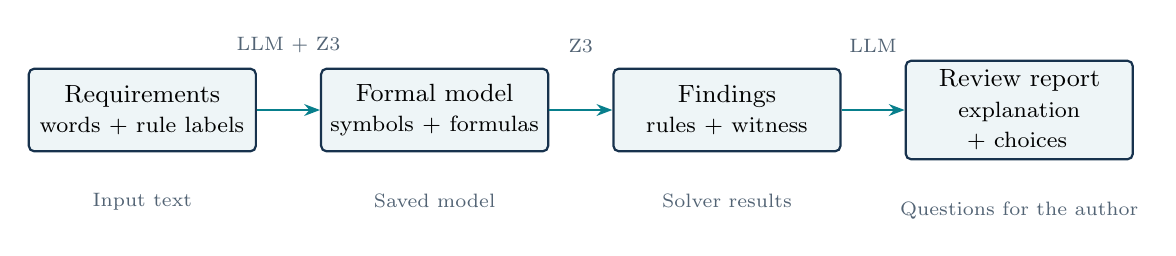
\begin{tikzpicture}[node distance=8mm]
\node[stage] (words) {Requirements\\\footnotesize words + rule labels};
\node[stage,right=of words] (formal) {Formal model\\\footnotesize symbols + formulas};
\node[stage,right=of formal] (finding) {Findings\\\footnotesize rules + witness};
\node[stage,right=of finding] (report) {Review report\\\footnotesize explanation + choices};
\draw[flow] (words)--node[above=6mm,annotation]{LLM + Z3}(formal);
\draw[flow] (formal)--node[above=6mm,annotation]{Z3}(finding);
\draw[flow] (finding)--node[above=6mm,annotation]{LLM}(report);
\node[annotation,below=4mm of words] {Input text};
\node[annotation,below=4mm of formal] {Saved model};
\node[annotation,below=4mm of finding] {Solver results};
\node[annotation,below=4mm of report] {Questions for the author};
\end{tikzpicture}
}
\caption{The three stages save their results separately. The solver stage makes no LLM calls.}\label{fig:pipeline}
\end{figure}

For authentication R3, the translation stage identifies the failed-attempt count and locked state. The solver finds that the lockout obligation cannot be obeyed together with the proposed administrator exception R5 at five failed attempts. The explanation stage returns the conflict and keep/change choices. Rule labels, formulas, assumptions and the witness remain available alongside the wording; the solver checks can be replayed without a model server.

\begin{table}[H]
\centering
\begin{tabularx}{\linewidth}{@{}lXX@{}}
\toprule
Responsibility & What it does & What it does not establish \\
\midrule
Language model & Extracts symbols and rules; proposes readings and assumptions; words findings & That the original author's intent was preserved \\
Python code & Chooses queries; clusters, votes, filters and combines results & A formal proof of the orchestration itself \\
Z3 & Returns satisfiability results, models and unsatisfiable cores for supplied formulas & Whether the symbols faithfully describe the real system \\
\bottomrule
\end{tabularx}
\caption{What each part of the system can establish.}
\end{table}

\subsection{Snapshot model}\label{sec:model}

Let $V$ be a finite vocabulary of Boolean, integer, real or finite-enumeration symbols. A valuation $\sigma$ assigns each symbol a value of its sort. It represents one snapshot of conditions, events and responses. There is no transition relation, trace, clock or built-in notion of \emph{previously}.

An atomic rule is $r_i=(a_i,c_i)$, with antecedent $a_i$ and consequent $c_i$. Its meaning is $\phi_i=a_i\Rightarrow c_i$; $\Phi=\bigwedge_i\phi_i$ denotes all retained rules. For the detailed solver examples, we now use the order case from Table~\ref{tab:order}. Its notation is local to that case: $s$ means submitted, $v$ means stock available, $f$ means fulfilled, $b$ means backordered, $c$ is a cancellation event, $q$ is the canceled-and-refunded state and $u$ means payments refunded. The standalone $c$ is distinct from the subscripted consequent $c_i$. The central rules are
\[
 \phi_1=(s\land v)\Rightarrow f,\qquad
 \phi_2=(s\land\neg v)\Rightarrow b,\qquad
 \phi_3=\True\Rightarrow\neg b.
\]
The complete five-rule model and its saved identifiers are in Appendix~\ref{app:formal-model}. The formulas use SMT-LIB syntax~\citep{smtlib} and are parsed into Z3 expressions; the checker does not execute arbitrary Python generated by the language model.

These definitions limit what a finding establishes. A conflict concerns the encoded obligations in an encoded situation. Whether the symbols capture the intended objects, timing and business rules remains a translation question.
\source{speccheck/logic.py; speccheck/checks.py; specs/order/formal.json}

\subsection{Translation and interpretation checks}\label{sec:formalize}

The first difficulty is choosing a vocabulary that preserves relationships between requirements. R2 and R3 must share the backorder symbol $b$; otherwise the contradiction becomes invisible. Extraction asks the model to preserve requirement IDs and source wording, and uses event markers to distinguish occurrences from states. Vocabulary validation checks names and sorts, but cannot verify that all requirements were found or that the abstraction is appropriate (Algorithm~\ref{alg:read}).

Repeated translation then asks whether the model gives a consistent reading within that vocabulary. The default is eight samples per rule at temperature 0.7. Z3 groups whole implications by equivalence. Here $\oplus$ is exclusive OR, and $\UNSAT$ means no satisfying assignment exists. The test proves that no assignment makes exactly one formula true; an unknown result proves neither equivalence nor inequivalence:
\[
 \phi\sim\psi\quad\Longleftrightarrow\quad\UNSAT(\phi\mathbin{\oplus}\psi).
\]
The largest group supplies the selected reading; the distribution over usable groups determines the initial accepted, ambiguous or rejected status. Rejected rules are reported for clarification and omitted from the main solver checks. Algorithms~\ref{alg:sample} and~\ref{alg:cluster} give the sampling, entropy thresholds and selection rules.

\example{A situation that distinguishes two readings.}
Let $n$ be the number of failed attempts. For ``lock the account when failed attempts reach five,'' $n=5$ and $n\ge5$ differ at six failed attempts with the account unlocked. That situation obeys the first implication and violates the second. In an illustrative eight-sample split, five readings of one kind and three of the other indicate disagreement; replacing $n=5$ with $5=n$ does not.

The pipeline uses such witnesses to ask focused questions about the original wording. It tests both presentation orders and retains answer counts, so the reviewer can see how a reading was challenged. Even unanimous preference for another reading is referred to the author; the implementation does not silently replace the requirement's meaning. Proposed alternatives still use the original vocabulary, so a missing meaning can remain undiscovered (Algorithm~\ref{alg:probe}).

An optional second model supplies another set of readings in the same vocabulary. Confirmation is conditioned on required event symbols, avoiding a spurious disagreement when a reader omits an explicit event guard. An unconfirmed accepted rule becomes ambiguous only when a usable alternative exists (Algorithm~\ref{alg:second-reader}). The second reader is off by default. Agreement within one model, agreement between models, and agreement across newly chosen vocabularies are different observations; none is a calibrated probability of correctness.
\source{speccheck/formalize.py; speccheck/probe.py}

\subsection{Relations between outcomes}

Boolean logic does not infer a relation from English names. Separate symbols for ``available'' and ``unavailable'' can both be true unless a formula relates them. The pipeline therefore asks for domain facts from symbol descriptions, without showing the requirements, and retains supported assumptions unless they are proved inconsistent with those already retained. These remain assumptions for the reviewer to assess (Algorithm~\ref{alg:facts}).

\example{Removal and retention.}
In the deletion case, let $d$ mean confirmation, $m$ removal and $k$ retention. The formulas $d\Rightarrow m$ and $k$ can coexist. If D2 is restated using the other outcomes while its private removal symbol is hidden, a supported reading $d\Rightarrow\neg k$ yields the assumed link
\[
 (d\land m)\Rightarrow\neg k.
\]
This can expose the clash with D4. It can also be wrong: ``remove'' may mean hiding a record while retaining an audit copy. The link procedure and subsequent probes preserve that qualification (Algorithms~\ref{alg:links} and~\ref{alg:probe}).

For rules whose triggering conditions are not proved incompatible, outcome-pair questions ask whether two definite outcomes, expressed with disjoint symbols, can coexist in one snapshot. The prompt does not include the triggering conditions. A majority of returned answers judging them incompatible adds the unguarded relation $\neg(c_i\land c_j)$ to the assumptions. The check skips disjoint events and already excluded pairs, and asks at most forty eligible pairs in document order. Solver unknown can leave a pair eligible; it does not prove compatible triggers. This mechanism is on by default in the frozen revision and is the subject of RQ1.
\source{speccheck/formalize.py; speccheck/probe.py}

\section{Findings}\label{sec:solver}

With an interpretation in place, the checker asks which obligations clash, which situations have no conditional response, and which allowed behaviours deserve review. The order example makes the distinction concrete: R2 and R3 conflict, an idle order may reasonably have no response, and fulfillment without submission may reveal a missing restriction.

\subsection{Conflicts}

Write $\SAT(F)$ for a satisfying solver result and $\UNSAT(F)$ for a proof that no satisfying assignment exists. Each query has a five-second timeout. An unknown result establishes neither. The search needs a feasible triggering situation as well as incompatible obligations.

For trigger group $G$, let $A_G=\bigwedge_{i\in G}a_i$. With an assumption set $B$, a conflict requires
\[
 \SAT\left(A_G\land\bigwedge B\right),\qquad
 \UNSAT\left(A_G\land\bigwedge B\land\Phi\right).
\]
For R2 and R3, $s\land\neg v$ is feasible, but it forces both $b$ and $\neg b$. Merely checking $\Phi$ would miss the problem: the solver can satisfy all five implications by choosing no submission or cancellation.

The search considers connected trigger groups of up to three rules and extracts a deletion-minimized unsatisfiable core only after an explicit unsatisfiable result. It excludes situations forbidden by one rule alone. The limit concerns trigger groups, not necessarily the number of rules in an explanation. A conclusive core is subset-minimal; it is not necessarily the smallest possible explanation, and the search does not enumerate every explanation (Algorithm~\ref{alg:conflicts}).

The checker runs first without assumptions, then with them. The second pass may add a conflict but cannot suppress one from the first; assumptions that exclude a rules-only trigger mark it doubtful. For example, assuming $\neg(f\land q)$ can make R1 alone forbid the submitted, in-stock, canceled-and-refunded situation. A rules-only pass preserves the R1/R5 clash for review instead of letting that assumption hide it.

\subsection{Gaps}
Let $C$ contain the rules with non-tautological antecedents. For an event $e$ to which a conditional rule reacts, the gap search seeks
\[
 e\land\bigwedge_{e'\ne e}\neg e'\land\bigwedge_{i\in C}\neg a_i.
\]
It returns at most one generalized example for each such event and one with no event. In change mode, a usable removed rule can seed the search with a situation it used to cover; that example takes priority for its selected event. At least one surviving conditional rule must still react to an event from the removed rule. Without reacted-to events, the fallback searches up to three generalized gaps, without removal attribution. If no conditional rule remains, it returns no gaps. Assumptions can mark a gap implausible but do not erase it; rejected translations can create apparent missing coverage (Algorithm~\ref{alg:gaps}).

In the order example, R1 and R2 cover submission with and without stock. The quiet case $s=c=q=\False$ has no conditional response, although R3 still forbids backordering; waiting may be intended. Removing R2 while retaining R1 leaves $s=\True,v=c=q=\False$ without a conditional response. This illustrates why event coverage is useful, while still being narrower than completeness of a business process.

\subsection{Scenarios}
For each rule, the allowed-scenario query is $\SAT(\Phi\land\neg a_i\land c_i)$. R1 says when fulfillment is required; it does not say ``only then.'' The model permits $s=c=q=b=\False$ with $f=\True$, so fulfillment without submission is a consequence for the author to review. A second search finds combined antecedents whose situation is forbidden by one rule alone. Both searches use the rules without domain assumptions. An LLM selects at most three consequences to discuss; offline replay without an LLM omits that presentation branch.
\source{speccheck/checks.py}

\subsection{Explanations and qualifications}\label{sec:explanation}

The explanation stage receives the finding, original requirements and an exact evidence sheet. It adds a title, explanation and keep/change choices. The witness and IDs remain available independently. An unparseable response leaves the finding unworded, while an API exception can still abort the run. The optional text review is off by default; its suggestions remain separate from solver findings.

The report also records sensitivity to alternative readings and vocabularies. It substitutes one ambiguous reading at a time and reruns the bounded checks; it does not test every combination. A gap annotation means that an alternative may cover part of the reported region, not that the whole gap disappears. Solver unknown can produce that hint, and a conflict absent from a bounded rerun does not prove consistency. Appendix~\ref{app:explanation} gives the counterexample and the rules for comparing multiple vocabularies.

All solver statements are conditional on the encoding. No proof certificate is archived, and generated prose is not formally checked. The R2/R3 result needs no assumed relation; a deletion conflict may depend on the removal/retention link; another finding may require simultaneous events. Reviewers need those distinctions alongside the explanation.
\source{speccheck/checks.py; speccheck/explain.py}

\section{Changes}\label{sec:change}

\subsection{Project baseline and proposed change}

OpenSpec keeps the project's existing behaviour under \code{openspec/specs/}. A proposed change has its own folder under \code{openspec/changes/}; its specification files describe the difference, or \emph{delta}, to apply to that baseline~\citep{openspec}. A capability such as authentication has the same relative path in both places. The checker loads the project's capability specifications, combines them with the selected change, and checks that combined document. It does not apply or archive the change in the source project.

The authentication example makes the layout concrete. These are the relevant files under \code{specs/auth_change/}:
\begin{lstlisting}
openspec/
|-- specs/auth/spec.md                     baseline
`-- changes/admin-never-locked/
    |-- proposal.md                       motivation
    `-- specs/auth/spec.md                delta
\end{lstlisting}

The \href{\authbaseurl}{baseline authentication specification on GitHub} contains the two requirements and four scenarios introduced in Table~\ref{tab:auth-baseline}. We return here to the authentication labels: R1--R4 are the existing scenarios in the combined full-mode document, and R5 is the proposed addition. These labels are separate from the order example's labels.

The \href{\authchangeurl}{proposed change on GitHub} adds one requirement. This is its literal specification text, with blank lines omitted:
\begin{lstlisting}
## ADDED Requirements
### Requirement: Administrator Access
Administrators MUST always be able to reach the system.
#### Scenario: Administrators are never locked out
- **WHEN** the account belongs to an administrator
- **THEN** the system does not lock the account
\end{lstlisting}

The four baseline scenarios remain \code{existing}; the administrator scenario becomes \code{added}, labelled R5 in this combined document. At five failed attempts, R3 requires locking an administrator's account under either threshold reading, while R5 forbids it. This particular conflict needs the base and the delta together. The saved findings also contain an older R1/R4 conflict: the checker retains it in the evidence but excludes it from the change report. The baseline is therefore not assumed to be free of defects.

\subsection{Applying the delta}

A delta file can use up to four operation sections. The checker applies them in the order shown in Table~\ref{tab:delta-operations}, regardless of their order in the file. Requirements are matched by name within their capability. A rename therefore takes effect before a removal or rewrite refers to the resulting name. References to missing requirements and additions of requirements already present are rejected (Algorithm~\ref{alg:change}).

\begin{table}[H]
\centering
\begin{tabularx}{\linewidth}{@{}llX@{}}
\toprule
Order & Section & What the delta supplies \\
\midrule
1 & \code{RENAMED} & A FROM/TO pair of requirement names; the requirement keeps its content under the new name. \\
2 & \code{REMOVED} & The name of an existing requirement. Text below that heading explains the reason for removal. \\
3 & \code{MODIFIED} & The full new requirement, including every scenario that should remain. \\
4 & \code{ADDED} & A new requirement's full text. ADDED can also create a specification for a capability with no baseline file. \\
\bottomrule
\end{tabularx}
\caption{The four operation headings have the form \texttt{\#\# ADDED Requirements}, with ADDED replaced by the appropriate operation.}\label{tab:delta-operations}
\end{table}

Within a MODIFIED requirement, scenario names identify which old and new scenarios correspond. The checker then compares their normalized bodies, ignoring case, extra whitespace and selected Markdown marks. Table~\ref{tab:scenario-status} gives the four possible states. These are textual classifications; they do not establish that a rewrite changes or preserves the intended meaning.

\begin{table}[H]
\centering
\begin{tabularx}{\linewidth}{@{}lX@{}}
\toprule
Scenario state & How it is assigned \\
\midrule
\code{existing} & The same name and normalized body remain, including inside a rewritten requirement. \\
\code{modified} & The name remains but the normalized body changes. \\
\code{added} & The scenario name is new, or its entire requirement is added. \\
\code{removed} & The whole requirement is removed, or its rewritten text omits an old scenario name. \\
\bottomrule
\end{tabularx}
\caption{Scenario provenance determines which findings are relevant to the change.}\label{tab:scenario-status}
\end{table}

For example, rewriting Account Lockout while retaining its Locked account scenario unchanged leaves that scenario \code{existing}. Changing only the Lockout threshold scenario makes that scenario \code{modified}. Omitting Locked account from the replacement text instead makes it \code{removed}. These are independent illustrations of the matching rules; the saved administrator change above only adds R5.

The default route formalizes the combined document, including removed scenarios labelled \code{X1}, \code{X2}, and so on. Before solver analysis, it separates the removed obligations and discards links or outcome-pair assumptions tagged with them. Ordinary voted facts remain. The removed obligations are no longer active rules, but their antecedents can guide a search for newly uncovered situations. Their text can still affect the full run's vocabulary and other assumptions.

\subsection{Removing a response}

\example{Removing the no-stock response.}
Take the order model and remove R2 while retaining R1. This is a constructed change to the order EARS example, not a saved OpenSpec order change. We use X1 for the removed R2 to explain the change-mode label. R1 still handles submission with stock. The situation $s=\True,v=c=q=\False$ now has no conditional response; R3 remains a prohibition, not a response. The removed rule's antecedent points directly to this missing branch.

\begin{figure}[H]
\centering
\resizebox{0.94\linewidth}{!}{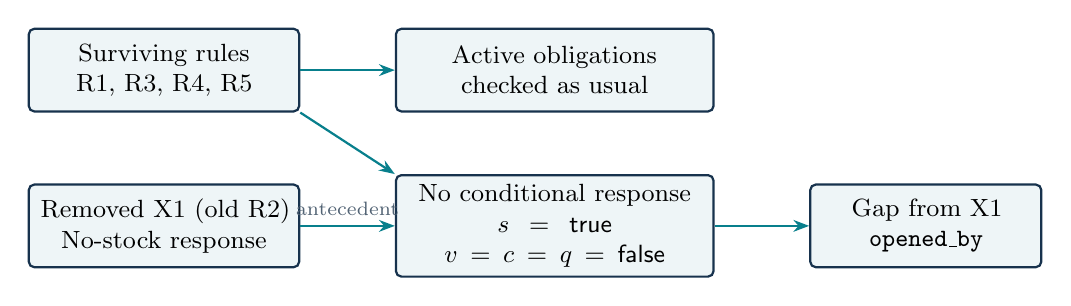
\begin{tikzpicture}[node distance=9mm and 12mm]
\node[stage,text width=3.2cm] (active) {Surviving rules\\R1, R3, R4, R5};
\node[stage,text width=3.2cm,below=of active] (removed) {Removed X1 (old R2)\\No-stock response};
\node[stage,text width=3.8cm,right=of active] (check) {Active obligations\\checked as usual};
\node[stage,text width=3.8cm,right=of removed] (seed) {No conditional response\\$s=\True$\\$v=c=q=\False$};
\node[stage,text width=2.7cm,right=of seed] (finding) {Gap from X1\\\texttt{opened\_by}};
\draw[flow] (active) -- (check);
\draw[flow] (active.south east) -- (seed.north west);
\draw[flow] (removed) -- node[annotation,above] {antecedent} (seed);
\draw[flow] (seed) -- (finding);
\end{tikzpicture}
}
\caption{The removed no-stock rule leaves the active model, but supplies the situation used to investigate a gap. The labels illustrate the order change.}\label{fig:removal}
\end{figure}

\begin{lstlisting}
{"type": "gap", "event": "order_submitted",
 "opened_by": ["X1"], "about_change": true}
\end{lstlisting}
These fields illustrate the attribution; they are not a literal saved order-change result. The change report includes this gap even though X1 is no longer an active obligation. If every response to submission is removed, the event is treated as retired and this search does not report a removal gap. State-only removals and rejected removed translations also fall outside this attribution mechanism. A gap associated with an added or modified rule's event is relevant to the change; that association alone does not prove the change caused it.

\subsection{Saved-base reuse}\label{sec:incremental}

The optional \code{--incremental} route formalizes the existing specifications once and retains that base model. It then translates only added or rewritten scenarios, labelled \code{N1}, \code{N2}, and so on, using the base vocabulary. Existing symbols and readings stay fixed. The pipeline probes the new rules and their eligible interactions with old rules, combines the models, removes deleted or replaced rules, and reruns the ordinary solver analyses. It reuses translation work; it does not incrementally update solver proofs (Algorithm~\ref{alg:incremental}).

\begin{figure}[H]
\centering
\resizebox{\linewidth}{!}{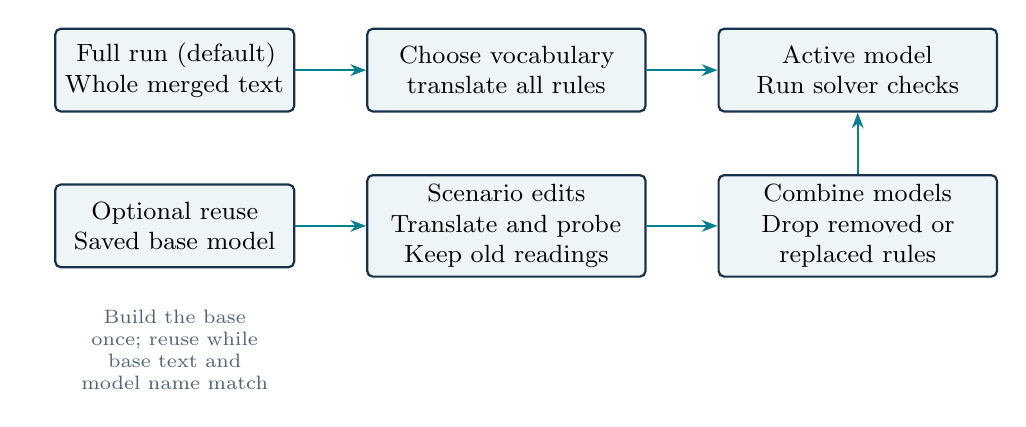
\begin{tikzpicture}[node distance=9mm and 9mm]
\node[stage,text width=2.8cm] (full) {Full run (default)\\Whole merged text};
\node[stage,text width=3.3cm,right=of full] (translate) {Choose vocabulary\\translate all rules};
\node[stage,text width=3.3cm,right=of translate] (analyze) {Active model\\Run solver checks};
\node[stage,text width=2.8cm,below=of full] (base) {Optional reuse\\Saved base model};
\node[stage,text width=3.3cm,right=of base] (new) {Scenario edits\\Translate and probe\\Keep old readings};
\node[stage,text width=3.3cm,right=of new] (combine) {Combine models\\Drop removed or\\replaced rules};
\draw[flow] (full) -- (translate);
\draw[flow] (translate) -- (analyze);
\draw[flow] (base) -- (new);
\draw[flow] (new) -- (combine);
\draw[flow] (combine) -- (analyze);
\node[annotation,below=4mm of base,text width=3.5cm] {Build the base once; reuse while\\base text and model name match};
\end{tikzpicture}
}
\caption{Two routes to the same analysis procedures. Their resulting encodings may differ, so the same solver checks do not establish equal detection quality.}\label{fig:incremental}
\end{figure}

For the administrator exception, the saved model supplies the lockout reading and vocabulary; only the new exception and its interactions need new translation questions. Repeated alternatives against the same base can share that initial work. Editing or archiving into the base specifications changes its text fingerprint and requires another base formalization. The cache also checks the model name, but not sampling settings, prompts, endpoint or code version. Invalid labels or an unusable model abort; there is no automatic fallback to a full merged-document run.

This mode currently follows scenario edits. Changing only a requirement's SHALL sentence while retaining the same scenarios, or adding a requirement without scenarios, can yield no new text and reuse the old model. Full mode is needed for those changes and for reconsidering existing interpretations. Incremental mode also excludes multiple vocabularies, a second reader and text review. E20 measures the resulting detection and request tradeoff; it does not establish equivalent semantic accuracy.
\source{speccheck/change.py; speccheck/cli.py}

\section{Evaluation}\label{sec:evaluation}

\subsection{Setup and measures}\label{sec:experimental-setup}

The experiments address the four research questions with separate comparisons. RQ1 uses the E18 outcome-pair ablation and the earlier T22 development-data comparison. RQ2 uses the E9 and E12 second-reader experiments. RQ3 uses E17's OpenSpec changes, E19's removal cases and E20's full-versus-reuse comparison. RQ4 uses the larger specification exercises and E20's formalization requests. The experiments differ in pipeline version and purpose, so their scores are reported separately.

The evaluation contains eleven sets of ordinary specifications: 66 base
documents in 297 versions. Separately, E17, E19 and E20 contain 18 OpenSpec projects with
102 distinct changes: 30, 36 and 36 respectively. E20 runs both modes on the same changes; it does not add another 36 cases. The scale exercises contain one 30-requirement and one
100-requirement document, each in four versions. These are project-authored
examples in Kiro EARS and OpenSpec formats. Most versions introduce one known
defect into a base document; the initial set also contains multiple planted
conflicts. The three original development examples are separate from this
inventory. Each evaluation version is run three times.
\source{research.md, sections 1 and 4.7; experiments/sets/}

The main model is \code{Qwen/Qwen3.8-27B-FP8}, served locally by vLLM. The
standard setting uses one symbol set, eight samples per translation or
question, and sampling temperature 0.7. E9 and E12 additionally evaluated
\code{thelamapi/next-70b} as a second reader. These are historical experiments
with different pipeline versions, not repeated measurements of one unchanged
system. Their saved JSON contains the specifications, expected defects, prompts,
formalizations and answers; the accompanying tables record solver scoring.

A conflict hit means the expected set of rule positions was reported. A gap
hit means a reported uncovered situation contains the event associated with
the planted missing case. This tests event coverage, not every possible missing
behaviour. Clean-run conflict alarms count runs with at least one unexpected
conflict; ambiguity flags count individual rules needing clarification,
including rejected translations. These quantities have
different denominators and should not be combined into an overall accuracy.
Repeated runs mainly expose translation instability: three runs of one defect
are not three independent requirements problems.
\source{experiments/evaluate.py, reported and gap_scores}


\subsection{Versions and reproducibility}
This report describes revision \code{498dea0}, preserved separately from the earlier \code{18752f2} edition. Historical experiments used different pipeline versions, and many older results do not identify the source commit that generated them. E19 evaluated the removal design frozen at \code{07ecd38}; E20 evaluated reuse at \code{373ae4c}. Their inputs were committed before those designs were frozen. E20 used one vocabulary, eight samples, temperature 0.7, three repetitions of 36 changes in each mode, and eighteen separately formalized bases. The model-name cache check, cache messages and second-reader/text-review option restrictions in the current revision were added after E20 and were not evaluated by those model runs.

The current offline suite passed 70 tests during preparation. These engineering checks are separate from the historical model experiments, which were inspected rather than rerun. Model weights and GPU services are external, so the saved results alone are insufficient to reproduce the original stochastic runs. A formalization request is one API call, which may return several samples; request counts are not sample counts or measured monetary cost.

\subsection{RQ1: conflicts and additional alarms}\label{sec:rq1}

We report detection counts alongside the additional findings that a reviewer would need to assess. Conflict alarms are counts of runs, ambiguity flags are counts of rules, and the scale observations are individual measurements.

E18 used six new domains---beds, timesheets, aquariums, cloakrooms, turbines and
payroll---with six versions each: clean, direct conflict, overlapping conflict,
two ambiguities, and a gap. The set was committed before the design was frozen.
The 108 runs contain 36 planted conflict opportunities and 18 clean runs.
The comparison in Table~\ref{tab:e18} scores the \emph{same saved runs} with and
without the facts added by the outcome-pair questions. It therefore isolates
that addition without resampling the earlier formalization.

\begin{table}[H]
\centering
\small
\begin{tabularx}{\linewidth}{@{}Xrr@{}}
\toprule
E18 measure & Without questions & With questions \\
\midrule
Planted conflicts found & 27/36 & 34/36 \\
\quad Direct conflicts & 9/18 & 16/18 \\
\quad Overlapping conflicts & 18/18 & 18/18 \\
Clean runs with a conflict alarm & 0/18 & 3/18 \\
Unexpected conflicts, all versions & 1 & 28 \\
Planted ambiguities found & 16/36 & 16/36 \\
Planted gaps found & 17/18 & 17/18 \\
Clean runs with a gap on a covered event & 0/18 & 0/18 \\
\bottomrule
\end{tabularx}
\caption{E18: default scoring, including doubtful conflicts. Removing doubtful
conflicts changes unexpected-conflict counts to 0 and 27; the other entries
are unchanged. Counts of findings and counts of runs are distinct.}
\label{tab:e18}
\end{table}

\begin{figure}[H]
\centering
\begin{minipage}{0.48\linewidth}
\centering
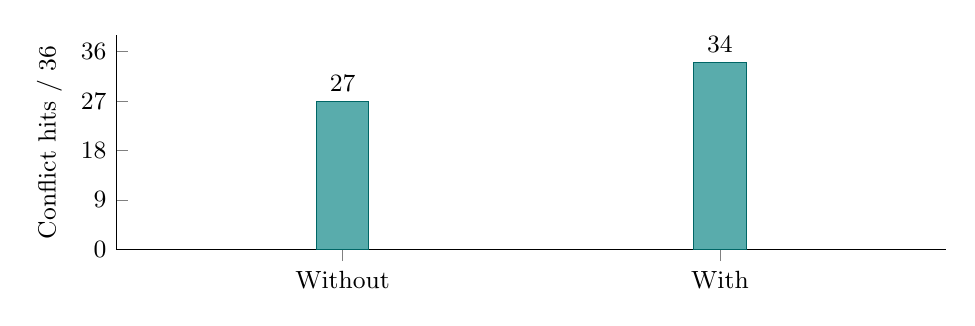
\begin{tikzpicture}
\begin{axis}[width=\linewidth,height=4.3cm,ybar,bar width=19pt,
  ymin=0,ymax=39,ytick={0,9,18,27,36},xmin=-0.6,xmax=1.6,
  xtick={0,1},xticklabels={Without,With},
  ylabel={Conflict hits / 36},tick label style={font=\small},
  label style={font=\small},nodes near coords,
  every node near coord/.append style={font=\small},
  axis lines*=left,enlarge x limits=false]
\addplot[fill=teal!65,draw=teal!80!black] coordinates {(0,27) (1,34)};
\end{axis}
\end{tikzpicture}
\end{minipage}\hfill
\begin{minipage}{0.48\linewidth}
\centering
\begin{tikzpicture}
\begin{axis}[width=\linewidth,height=4.3cm,ybar,bar width=19pt,
  ymin=0,ymax=19.5,ytick={0,3,6,9,12,15,18},xmin=-0.6,xmax=1.6,
  xtick={0,1},xticklabels={Without,With},
  ylabel={Clean alarm runs / 18},tick label style={font=\small},
  label style={font=\small},nodes near coords,
  every node near coord/.append style={font=\small},
  axis lines*=left,enlarge x limits=false]
\addplot[fill=orange!65,draw=orange!80!black] coordinates {(0,0) (1,3)};
\end{axis}
\end{tikzpicture}
\end{minipage}
\caption{The E18 tradeoff. ``With'' means the outcome-pair questions are
included. Each axis states its own denominator; these are different measures.}
\label{fig:e18-tradeoff}
\end{figure}

\example{A conflict recovered: releasing and holding a hospital bed}
The original translation used separate symbols for releasing a bed and holding
it for 24 hours. Z3 could satisfy both. All eight answers to the outcome
question judged them incompatible, supplying the missing assumed fact. The
planted conflict was then found in all three runs. Retention wording in the
cloakroom case was similarly recovered. Across E18, 410 pairs were asked about
and 58 received a majority of ``impossible'' answers.
\source{research_log.md, E18; experiments/results/E18_eval12.json}

\example{A conflict still missed: retaining payroll records}
``Keep every payslip for ten years'' sometimes became merely
\code{payslip_retention_years = 10}. Nothing in that formula prevents deletion.
One run supplied the missing connection, another split four votes to four,
and a third expressed conditional retention rather than one definite outcome,
so the pair was not asked about. The direct payroll conflict was found in only
one of three runs. More samples do not automatically repair the choice of symbols.

\example{The cost: collecting a coat that was previously unclaimed}
A clean cloakroom specification says to release a coat when a guest presents
its token, and to list coats left for over 30 days as unclaimed. The one-snapshot
model treats release and being unclaimed as incompatible simultaneous outcomes.
A perfectly ordinary history---list the coat first, release it later---has been
collapsed. This one pair accounts for 24 of the 27 additional unexpected
conflicts across versions, including all three clean-run alarms. The remaining
three additional findings involve a planted timesheet rule and a third rule.
The unexpected findings therefore need individual review. In the cloakroom
case, the alarm comes from collapsing successive states into one snapshot.
\source{research_log.md, E18; experiments/results/E18_eval12.md}

The earlier T22 development-data ablation supports the same tradeoff: on saved
models from eight older sets, conflict hits rose from 132/153 to 145/153.
With doubtful findings excluded, the corresponding values were 129/153 and
142/153, while clean alarm runs rose from 3/144 to 13/144. Those results
motivated the design; they remain separate from the held-out E18 evidence.
\source{research_log.md, T22}

\subsection{RQ2: ambiguity and review questions}\label{sec:rq2}

\begin{table}[H]
\centering
\small
\begin{tabular}{@{}lrr@{}}
\toprule
Measure & Main model & With second reader \\
\midrule
E9: planted ambiguities & 14/36 & 30/36 \\
E9: clean-spec rule flags (18 runs) & 7 & 15 \\
E12: planted ambiguities & 17/36 & 32/36 \\
E12: clean-spec rule flags (18 runs) & 5 & 9 \\
\bottomrule
\end{tabular}
\caption{Second-reader results on two separate 72-run experiments. Rule flags
are counts, not percentages of clean runs.}
\label{tab:second-reader-evaluation}
\end{table}

\example{Does ``if'' govern the gate, the photograph, or both?}
The ski-pass example requires the system to ``open the gate and show the
skier's photo if the pass is a season pass''. A reader can attach the condition
to the photograph alone or to both actions. A second model is more likely to
disagree with the first model's confident choice. Table~\ref{tab:second-reader-evaluation}
shows the resulting gain, together with additional review work. The clean-spec
flags are unplanted ambiguities whose correctness has not been independently
labelled, so we cannot count them all as false positives.
\source{experiments/sets/eval7/skipass_ambiguity2/spec.md; experiments/results/E9_eval4.md; experiments/results/E12_eval7.md}

\subsection{RQ3: changes and reuse}\label{sec:rq3}

E17 evaluates a different question: can the system apply an OpenSpec change,
preserve scenario identity, and report findings involving that change? Across
90 runs it found all 36 planted conflicts and all 36 planted gaps, with no
unexpected conflict or covered-event gap reported about the 18 clean changes.
Excluding doubtful conflicts reduces the conflict count to 33/36. All 90 runs
preserved the generated scenario labels.

\example{A cinema change stops seat sales when the projector fails}
The change modifies the operations specification to prohibit sales while a
hall's projector is out of order. The existing screenings specification still
requires a sale when a customer requests an available seat. Checking the merged
document exposes that interaction across files. In all three runs, however,
the projector's state was modelled as an event, making the conflict doubtful.
Filtering doubtful findings therefore loses this planted case.

The conflict wording in E17 deliberately negates an existing outcome directly.
The results support merging, labels and finding selection; they leave harder
semantic translations untested. At the time, removal-only gaps were not attributed to their
change, every scenario under a modified requirement counted as changed, and each
change required full formalization. E19 and E20 evaluate later changes to those behaviours.
\source{experiments/results/E17_eval11.md; research.md, sections 2.4 and 4.5}

\paragraph{E19: removals and unchanged scenarios.}
The next six projects contain 36 changes, each run three times. These cases include removing a whole requirement, dropping a scenario, narrowing coverage, retiring an event, and modifying one scenario while leaving its siblings unchanged. Table~\ref{tab:e19} separates the planted defects from quiet changes. The 54 quiet-change runs include clean, retirement and unchanged-sibling cases; their denominator differs from E17's 18 clean runs.

\begin{table}[H]
\centering
\small
\begin{tabularx}{\linewidth}{@{}Xr@{}}
\toprule
E19 measure & Result \\
\midrule
Planted conflicts found & 18/18 \\
\quad After excluding doubtful findings & 15/18 \\
Planted gaps found & 35/36 \\
\quad Whole-requirement removals & 18/18 \\
\quad Dropped scenarios or narrowed coverage & 17/18 \\
Quiet-change runs with a conflict alarm & 2/54 \\
Quiet-change runs with a gap alarm & 0/54 \\
Runs preserving scenario labels & 108/108 \\
\bottomrule
\end{tabularx}
\caption{E19: removal handling and more precise scenario provenance.}
\label{tab:e19}
\end{table}

All eighteen event-retirement runs stayed quiet. Existing conflicts were found and excluded from the change report in all 108 run opportunities, covering six distinct old conflicts. In the missed narrowed-coverage case, the translation of a retained rule lost a condition and appeared to cover the missing branch. The two quiet-change conflict alarms involved reworded scenarios: textual change tracking cannot establish that a rewrite has the same meaning. These results support the new attribution mechanism on the tested cases, not complete regression detection.
\source{experiments/results/E19_eval13.md; research_log.md, E19}

\paragraph{E20: full formalization versus a saved base.}
E20 uses six further projects and 36 distinct changes, with three repetitions per mode. Each repetition includes eighteen planted-conflict, twelve planted-gap and six clean changes. The full mode chooses a vocabulary and translates the combined document; reuse keeps the base vocabulary and readings and translates the changed scenarios. Both then run the ordinary solver checks on their resulting encodings.

\begin{table}[H]
\centering
\small
\begin{tabularx}{\linewidth}{@{}Xrr@{}}
\toprule
E20 measure & Full & Reuse \\
\midrule
Planted conflicts found & 54/54 & 50/54 \\
\quad After excluding doubtful findings & 51/54 & 45/54 \\
Planted gaps found & 36/36 & 36/36 \\
Clean-change runs with conflict or gap alarms & 0/18 & 0/18 \\
Other change-related conflicts & 3 & 1 \\
Unplanted ambiguity flags & 1 & 4 \\
All change-related gaps & 39 & 42 \\
Runs preserving scenario labels & 108/108 & 108/108 \\
\bottomrule
\end{tabularx}
\caption{E20: detection changes when a saved interpretation is reused. Clean-run quietness does not mean that every other finding was a planted defect.}
\label{tab:e20}
\end{table}

\example{A new rule is read with a narrower trigger.}
In the driving-school case, a new rule about a person younger than seventeen sometimes acquired an unspoken registration-event condition when translated against the saved base. Disagreement or selection of a non-conflicting reading then lost the planted overlap conflict. The four missed run opportunities concern two distinct changes: this case in all three repetitions, and a brewery conflict in one. Reusing the base saves translation work but can alter how the new text is understood. The request savings are reported under RQ4; these data do not establish equal accuracy between the modes.
\source{experiments/results/E20_eval14_full.md; experiments/results/E20_eval14_incremental.md; research_log.md, E20}

\subsection{RQ4: scale and cost}\label{sec:rq4}

\paragraph{Requests saved by reusing a base.}
E20 recorded the API requests and tokens used by the formalization stage. The measurements exclude the CLI's later explanation and scenario-judging calls. Table~\ref{tab:reuse-cost} separates the initial base build from each subsequent change.

\begin{table}[H]
\centering
\small
\begin{tabularx}{\linewidth}{@{}Xrrr@{}}
\toprule
Mean formalization usage & Full change & Reused-base change & Initial base \\
\midrule
API requests & 68 & 9 & 61 \\
Prompt tokens & 32,431 & 4,934 & 28,641 \\
Completion tokens & 28,806 & 3,816 & 25,969 \\
\bottomrule
\end{tabularx}
\caption{E20: rounded means. The base cost is additional and can be shared only while that base remains reusable. One request can return eight samples.}
\label{tab:reuse-cost}
\end{table}

The recorded totals were 7,336 requests for full runs, 1,010 for changes using saved bases, and 1,093 for eighteen base builds. Including those builds, reuse used 2,103 requests, about 71\% fewer in this experiment with six alternative changes per base. Excluding base builds gives about 86\% fewer. Neither percentage is an end-to-end CLI cost or a monetary saving. Archiving a change into the base forces a new build; one check after each archive therefore has a different cost profile. A removal-only change may need no new formalization calls while still requiring LLM calls to explain its findings.

The recorded batch times were about 32 minutes for full mode and 13 minutes for reuse including bases. These are observations from one batch setup, not per-change latency estimates. The conflict-detection loss in Table~\ref{tab:e20} is part of the same comparison and should accompany the savings.
\source{experiments/results/E20_eval14_full.md; experiments/results/E20_eval14_incremental.md; experiments/evaluate.py; research_log.md, E20}

\paragraph{Larger specifications.}

For the 30-requirement campsite document, skipping combinations from unrelated
rule families reduced solver time from 26--34 seconds to 0.4--0.9 seconds on
the saved models. Booking, barriers, showers and billing share few symbols.
Both planted conflicts were found in all three repetitions, as was the gap.
Each clean run had a doubtful conflict; excluding doubtful findings left none.
A densely connected document need not obtain the same speedup.

The 100-requirement ferry example required a larger read-output allowance:
one measured answer contained 16,799 tokens. All 12 runs then read the correct
number of requirements in their respective variants. Conflict hits were 6/6,
gap hits 3/3, and one of three clean runs had a conflict alarm. The culprit was
reserving a new seat versus releasing an old unpaid reservation: one state
variable represented different seats at different times. As in the cloakroom
example, the representation fails to distinguish states at different times;
here it also conflates separate objects.

One 101-rule model took 35 seconds in the solver; one full CLI run including
wording took 620 seconds on a busy cluster server. These are observations,
not latency averages. E18's 24 minutes for 108 runs on two GPUs is a separate
batch-throughput measurement. The current second-reader server cannot fit the
long ferry prompt under its configured prompt-plus-answer allowance, and the
outcome check asks only the first 40 eligible pairs on large documents.
\source{research_log.md, E13, E14 and E18}


\section{Limitations and next steps}\label{sec:discussion}

The results show that translation and representation choices determine which problems reach the solver. Outcome-pair questions recover relations that separate symbols can hide, but the cloakroom alarms show what happens when the representation collapses successive states. The payroll miss shows a different failure: a retention duration alone does not encode an obligation to keep the record. These cases explain why additional samples and stronger solver checks cannot by themselves guarantee faithful translation.

\subsection{Current capabilities}

For RQ1, the E18 comparison supports keeping the outcome-pair questions available, with their assumptions shown to the reviewer. They remain on by default in this revision. For RQ2, the second reader finds more planted ambiguities and also asks more questions about clean specifications. Their correctness has not been independently adjudicated. The two mechanisms add review work as well as detections.
\source{plan.md, section 3; research_log.md, E18}

RQ3 supports checking proposed changes in context and attributing tested removal gaps to the removed rules. E19 also shows why unchanged scenarios should keep their original provenance. E20 adds a practical tradeoff: keeping a base interpretation reduces repeated translation requests, but loses four of 54 planted-conflict run opportunities relative to full mode. Full formalization therefore remains the default. RQ4 shows that the prototype can process the tested larger documents and that reuse can reduce formalization work; it does not establish a general latency or capacity limit. Shared symbols, input allowance and the representation of objects and time all affect the result.
\begin{table}[H]
\centering
\begin{tabularx}{\linewidth}{@{}lXX@{}}
\toprule
Capability & Evidence now & Remaining limitations \\
\midrule
End-to-end checking & Saved models, findings and reports; order and deletion examples & Translation and explanation can still misstate intent. \\
Interpretation checks & Sampling, probes, optional second model & Shared vocabulary and correlated errors remain. \\
Change checking & E17, E19; removed-rule gap attribution & Event retirement, state-only removals, large real projects. \\
Saved-base reuse & E20; fewer requests, some missed conflicts & Scenario-only edit selection; fixed old readings; cache scope. \\
Engineering checks & 70 offline tests passed during preparation & Tests do not prove the orchestration correct. \\
Evaluation & Held-out-at-the-time sets, ablations, repeated runs & Project-authored data, limited model diversity. \\
\bottomrule
\end{tabularx}
\caption{Current capabilities, supporting evidence and remaining limitations.}
\end{table}

\subsection{Limits of reuse}

A saved model retains decisions as well as computation. Existing symbol definitions and rule readings are fixed, even when a new requirement would make another vocabulary preferable. New facts and links are checked selectively; the pipeline does not ask every old interpretation question again. The driving-school miss is a concrete reason to retain the full route and show the detection loss alongside request savings.

The implementation also selects incremental text by scenario changes. An edit confined to the requirement's SHALL sentence can be recorded as changed text but supply no new translation input. If extraction previously created a separate unlabelled rule for that sentence, a later sentence rewrite does not itself retire that old rule. The present mode therefore needs a narrower claim than arbitrary requirement-edit support. A full run includes the revised sentence.

Cache validity currently means matching generated base text and model-name strings. It does not verify sampling settings, endpoint, model weights, prompts or code version. Rebuilding a missing or mismatched base still uses the reuse route for the proposed change; it does not automatically choose full merged-document formalization. These are limits of the current implementation, not effects established by E20. They need explicit cases in the next evaluation.

\subsection{Validity and generalization}

The immediate use case is assisted requirements review, where reviewers can
examine the witnesses and assumptions. The evidence does not yet establish
production defect rates, human review savings, or sound translation of natural
language. Most documents and all planted defects were written by the project;
one earlier prompt example overlapped a held-out domain. Every inspected set
is now development data, so another design change needs a fresh set written
before that change is made.

The next evaluation should prioritize independently sourced specifications and
labels, another main model, and results per distinct defect alongside repeated
runs. Temporal and entity distinctions deserve targeted cases such as the
coat and seat examples. Scenario usefulness, explanation faithfulness and
irreducible three-rule conflicts also need dedicated evaluation. Existing
results justify continuing the prototype and identify where more work is
needed. Doubtful and assumption-dependent findings should remain visible to
reviewers.
\source{plan.md, section 2; research.md, sections 4.4--4.7; speccheck/change.py; speccheck/cli.py}

\subsection{Next steps}\label{sec:next}

The prototype turns a translated specification into review questions with solver evidence. The order example gives the author R2 and R3, a feasible no-stock submission, and incompatible obligations. For deletion, the reviewer also needs the assumed relation between removal and retention. Assumptions and alternative readings remain part of the review.

The experiments support continuing this approach with qualifications. Outcome-pair questions and a second reader improve detection while adding review work. Change checking now attributes tested removal gaps and offers saved-base reuse. E20 shows fewer requests alongside lower conflict detection, so full formalization remains the default. Input, runtime and representation limits remain; production accuracy and human review savings have not been established.

\paragraph{Independent evaluation.} Prepare a fresh set before another design change; the current sets have informed development. Add independently authored requirements and a real OpenSpec project's history. Report distinct defects as well as repeated runs, retain raw and doubtful-filtered findings, and measure review time. Record the requirements, reviewer decisions and fixed configuration so others can assess the results.

\paragraph{Change analysis on larger projects.} Test sentence-only edits, requirements without scenarios, state-only removals, and changes to old vocabulary meanings. Fix or reject unsupported edits explicitly. Compare repeated alternatives against one base with rebuilding after each archive; test cache validity across sampling, prompt and model changes. Investigate the E20 misses on fresh cases and measure context limits on a real project. The order removal remains a useful regression example: submission stays in scope while its no-stock branch is removed.

\paragraph{Vocabulary and representation.} Use the cloakroom failure and payroll miss as design cases: express retention as an obligation, test the outcome-pair cap, and investigate a doubt marker for collapsed lifecycles. Preserve contradictions such as order backordering while testing changes on fresh cases. The model remains one snapshot; a temporal extension has not been agreed. Reviewers still need to see where time and separate objects have been collapsed.

The order of work is evaluation, change analysis, then vocabulary selection. These are research priorities, without a staffing estimate or delivery schedule.
\source{plan.md, sections 2 and 5; research.md, sections 4 and 5}


\clearpage
\bibliographystyle{plainnat}
\bibliography{references}
\clearpage
\appendix
\section{The full order model}\label{app:formal-model}

A rule is $r_i=(a_i,c_i)$ with logical meaning $\phi_i=a_i\Rightarrow c_i$; $\Phi$ is the conjunction of the retained rule formulas. A valuation assigns every symbol one value in a single snapshot.
For the order example, we use the following abbreviations alongside the identifiers saved in the formal model.

\begin{table}[H]
\centering
\begin{tabularx}{\linewidth}{@{}clX@{}}
\toprule
Symbol & Saved identifier & Meaning \\
\midrule
$s$ & \code{order_submitted} & A submission event occurs. \\
$v$ & \code{inventory_available} & Stock is available. \\
$f$ & \code{order_fulfilled} & The order is fulfilled. \\
$b$ & \code{order_on_backorder} & The order is backordered. \\
$c$ & \code{order_canceled} & A cancellation event occurs. \\
$q$ & \code{order_canceled_and_refunded} & The canceled-and-refunded state holds. \\
$u$ & \code{payments_refunded} & The payments are refunded. \\
\bottomrule
\end{tabularx}
\caption{Stable abbreviations for the order worked example. All seven symbols are Boolean.}
\end{table}

An atomic rule is $r_i=(a_i,c_i)$, with antecedent $a_i$ and consequent $c_i$. Its logical meaning is $\phi_i=a_i\Rightarrow c_i$. The subscripted $c_i$ means a rule's consequent; the standalone $c$ in the order example is its cancellation event. With $\Phi=\bigwedge_i\phi_i$, the five rules become
\begin{align*}
\phi_1&=(s\land v)\Rightarrow f,&
\phi_2&=(s\land\neg v)\Rightarrow b,\\
\phi_3&=\True\Rightarrow\neg b,&
\phi_4&=c\Rightarrow u,\\
\phi_5&=q\Rightarrow\neg f.&&
\end{align*}

The persisted formulas use SMT-LIB syntax~\citep{smtlib}. For example, R2 is written as an antecedent \code{(and order_submitted (not inventory_available))} and a consequent \code{order_on_backorder}. The vocabulary object parses these strings and constructs Z3 expressions. The checker is not interpreting arbitrary Python generated by the language model.
Appendix~\ref{app:walkthrough} shows how the saved requirement, symbol, translation and finding correspond.

\source{speccheck/logic.py; speccheck/checks.py; specs/order/formal.json}

\subsection{Solver queries and assumptions}

Write $\SAT(F)$ when the solver returns a satisfying assignment for $F$, and $\UNSAT(F)$ when it establishes that no such assignment exists. The implementation also allows an \emph{unknown} answer, including on timeout. Unknown establishes neither result. Each solver query has a five-second timeout; the sensitivity annotations discussed later need an additional qualification.

We repeatedly use three patterns:
\begin{align}
\text{Equivalence: }&\quad \UNSAT(\phi\oplus\psi),\label{eq:equivalence}\\
\text{Entailment: }&\quad \UNSAT(B\land\neg d),\label{eq:entailment}\\
\text{Incompatibility in a context: }&\quad \UNSAT(T\land\Phi).\label{eq:incompatibility}
\end{align}
Here $B$ is a conjunction of assumptions, $d$ is a candidate consequence, and $T$ describes a triggering context. If the equivalence query is satisfiable, its assignment shows how the two readings differ. If the incompatibility query is unsatisfiable, we still need to check that $T$ itself is feasible before calling the result a conflict.

\example{Why simply checking all five rules is insufficient.}
Set $s=c=q=\False$ and $b=\False$. The conditional rules impose no demands, R3 is obeyed, and $\Phi$ is satisfiable. That does not resolve the backorder problem. Set $T=s\land\neg v$ instead. Now R2 forces $b$ and R3 forces $\neg b$. We have $\SAT(T)$ but $\UNSAT(T\land\Phi)$. The triggering context is what turns a vague global consistency question into the concrete problem we wanted to expose.

\subsection{Assumptions are not requirements}

Let $B$ hold relations proposed by the language model, such as a possible connection between removal and retention. These formulas can help reveal conflicts that the chosen symbols otherwise hide. They can also be wrong. The implementation first searches for conflicts using the rules alone, then searches with assumptions and labels any additional findings that depend on them. Assumptions may cast doubt on a rules-only finding; they must not silently remove it.

\example{An assumption can hide a clash between requirements.}
Suppose an assumed fact says that fulfillment and the canceled-and-refunded state never coexist: $\neg(f\land q)$. The trigger $s\land v\land q$ is still feasible. But under that assumption, R1 alone becomes impossible to obey there: it demands $f$ while the assumption forbids it. An assumptions-only pass would classify the case as a situation forbidden by one rule, rather than report the R1/R5 clash. Running the requirements-only check first preserves that clash for the author to inspect. The policy question stays visible.

Z3 checks the formulas it receives. To assess a finding, we need to know which formulas came from translated requirements, which came from assumed relations, and which interpretation choices affect the conclusion.
\source{speccheck/logic.py; speccheck/checks.py; specs/order/formal.json}


\clearpage
\section{Detailed procedures}\label{app:procedures}

This appendix gives the eleven procedures behind Sections~\ref{sec:design}--\ref{sec:change}, together with their voting rules, failure cases and sensitivity checks. The formulas and constructed sample distributions are explanatory examples, not additional experimental measurements. The seven translation steps describe the full route; Algorithm~\ref{alg:incremental} identifies which work the optional reuse route repeats.
\begin{figure}[H]
\centering
\resizebox{\linewidth}{!}{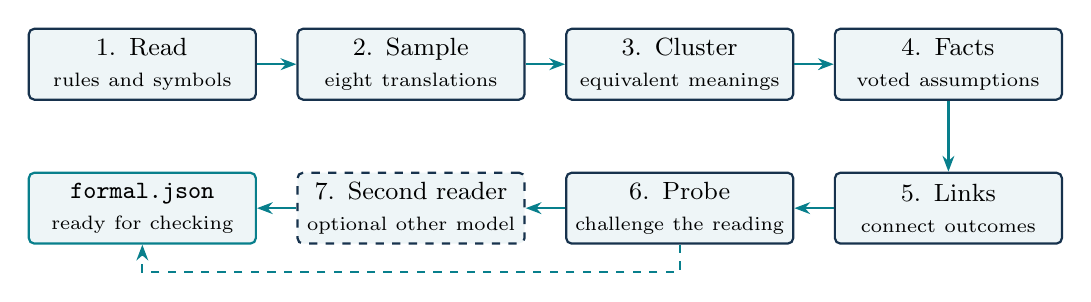
\begin{tikzpicture}[node distance=5mm,stage/.append style={text width=2.65cm,minimum height=9mm}]
\node[stage] (r) {1. Read\\\scriptsize rules and symbols};
\node[stage,right=of r] (s) {2. Sample\\\scriptsize eight translations};
\node[stage,right=of s] (c) {3. Cluster\\\scriptsize equivalent meanings};
\node[stage,right=of c] (f) {4. Facts\\\scriptsize voted assumptions};
\node[stage,below=9mm of f] (l) {5. Links\\\scriptsize connect outcomes};
\node[stage,left=of l] (p) {6. Probe\\\scriptsize challenge the reading};
\node[stage,left=of p,dashed] (x) {7. Second reader\\\scriptsize optional other model};
\node[stage,left=of x,draw=Teal] (o) {\texttt{formal.json}\\\scriptsize ready for checking};
\draw[flow] (r)--(s);\draw[flow] (s)--(c);\draw[flow] (c)--(f);
\draw[flow] (f)--(l);\draw[flow] (l)--(p);\draw[flow] (p)--(x);\draw[flow] (x)--(o);
\draw[flow,dashed] (p.south) -- ++(0,-.35) -| (o.south);
\end{tikzpicture}
}
\caption{The internal formalization flow. The dashed shortcut skips the optional second reader.}\label{fig:seven}
\end{figure}

\subsection{Translation and interpretation checks}\label{app:formalize}

For the order example, the translation must preserve the clash between
``backorder when there is no stock'' and ``never backorder.'' A solver can
establish that conflict once it receives the right formulas. Getting those
formulas is the harder part. The seven steps below produce and check the
translation before the solver analysis in Figure~\ref{fig:pipeline}.

We use the notation of Section~\ref{sec:model}: a rule is
$r_i=(a_i,c_i)$, with formula $\phi_i=a_i\Rightarrow c_i$, over vocabulary
$V$. The order symbols are $s$ (submitted), $v$ (stock available), $f$
(fulfilled), $b$ (backordered), $c$ (cancellation event), $q$
(cancelled-and-refunded state), and $u$ (refund). Short formulas and
constructed sample distributions below are illustrations of the algorithms,
not additional experimental measurements.

\subsubsection{Step 1: read the requirements and choose the vocabulary}
\example{One event, one condition, one demanded outcome}
For R2, ``WHEN an order is submitted AND inventory is unavailable, THE
Order System SHALL place the order on backorder,'' the reader must identify
the submission event $s$, the stock condition $v$, and the outcome $b$.
R3 must reuse $b$ when it says never to backorder. If the reader invents
unrelated symbols for these two mentions, the contradiction becomes
invisible to the solver.

\textbf{Input:} the original document.
\textbf{Output:} atomic requirements with IDs, source text and triggers,
plus typed symbols with descriptions. The supported sorts are Boolean,
integer, real and finite enumeration. Event markers distinguish an
occurrence, such as submission, from a state, such as being refunded.
The model is instructed to copy requirement text and preserve existing
labels; it does not receive a hand-written domain vocabulary.

\begin{algorithm}[H]
\caption{Read a document into rules and symbols}\label{alg:read}
\begin{algorithmic}[1]
\Require Document $D$, initial temperature $t$
\For{$\tau$ in $(t,0.3,0.9)$}
  \State Ask for atomic rules, triggers and symbols at temperature $\tau$
  \If{a JSON answer exists and its vocabulary is valid}
    \State \Return rules and vocabulary
  \EndIf
\EndFor
\State Fail with the extraction error
\end{algorithmic}
\end{algorithm}

Validation rejects illegal or duplicate symbol names, unsupported sorts,
and enumerations with fewer than two values. It does not establish that
the reader found every requirement or chose the intended abstraction.
A valid vocabulary can still encode the wrong meaning. The extraction
answer can also exceed the configured
token budget on a long document.
\source{speccheck/formalize.py}

\subsubsection{Step 2: translate each rule several times}
\example{Eight attempts to express the same obligation}
For R2, a translation may return $a_2=s\land\neg v$ and $c_2=b$.
Another may write an equivalent implication with a different syntactic
arrangement. The next step must compare meanings, rather than count
identical strings. For an authentication rule, repeated translations may
instead expose a real distinction: ``reaches five failed attempts'' can
be rendered using $n=5$ or $n\ge5$.

\textbf{Input:} one extracted requirement and the shared vocabulary.
\textbf{Output:} up to $N$ translations, each containing a plain-language
reading, an antecedent and a consequent. The defaults are $N=8$ and
sampling temperature $0.7$. Each call is constrained to a JSON schema;
the formulas themselves are subsequently parsed by Z3.

\begin{algorithm}[H]
\caption{Sample translations in a fixed vocabulary}\label{alg:sample}
\begin{algorithmic}[1]
\Require Rules $R$, vocabulary $V$, sample count $N$
\ForAll{$r_i\in R$ in parallel}
  \State Ask for $N$ translations of the text of $r_i$ using $V$
  \State Store the returned JSON answers for $r_i$
\EndFor
\State \Return sampled translations
\end{algorithmic}
\end{algorithm}

Up to sixteen requests are issued concurrently. Only the LLM calls run in
these worker threads; the subsequent Z3 work is serial. Invalid JSON
answers are dropped. Multiple samples provide evidence about variation
within a model, but they are not independent human judgments. A model can
repeat the same mistaken reading eight times.
\source{speccheck/formalize.py}

\subsubsection{Step 3: group translations by meaning}
\example{Agreement, a split, and scattered readings}
Suppose eight constructed samples of the authentication rule divide into
five translations using $n=5$ and three using $n\ge5$. The two meanings
disagree when $n=6$ and the account is not locked. That assignment obeys
the first implication and violates the second. By contrast, replacing
$n=5$ with $5=n$ changes no meaning and creates no extra cluster.

\textbf{Input:} sampled translations and $V$.
\textbf{Output:} semantic clusters, a selected reading, and an initial
status. Two compiled translations belong together when
\[
 \phi\sim\psi
 \quad\Longleftrightarrow\quad
 \UNSAT(\phi\mathbin{\oplus}\psi).
\]
The comparison concerns whole implications, not their antecedents and
consequents separately. For cluster sizes $m_1,\ldots,m_k$, the code uses
\[
 p_j=\frac{m_j}{\sum_\ell m_\ell},\qquad
 H=-\sum_j p_j\ln p_j.
\]

\begin{algorithm}[H]
\caption{Cluster and choose an initial reading}\label{alg:cluster}
\begin{algorithmic}[1]
\Require Sampled translations $T$
\State Discard translations that cannot be compiled
\State Group the rest by solver-proved equivalence
\If{no group remains} \State \Return rejected \EndIf
\State Compute $H$ from usable cluster sizes
\State Set status: accepted if $H\le0.4$; ambiguous if $H\le1$; else rejected
\State Select the shortest formula in the largest group
\State If not accepted, retain a second reading and a distinguishing witness
\end{algorithmic}
\end{algorithm}

Thus an illustrative $[8]$ or $[7,1]$ split is accepted, $[6,2]$ or
$[5,3]$ is ambiguous, and $[4,2,2]$ is rejected. These thresholds are
engineering choices. Entropy is computed over usable translations, so a
low value does not itself establish that many requested samples succeeded.
Later probes may change an accepted or ambiguous status. A rejected rule
is reported for clarification and excluded from the main solver checks.
\source{speccheck/formalize.py}

\subsubsection{Step 4: propose and vote on domain facts}
\example{Two names can describe mutually exclusive states}
The order model uses one stock variable $v$, so ``unavailable'' is simply
$\neg v$. If a vocabulary instead contains separate symbols
\code{stock_available} and \code{stock_unavailable}, Boolean logic alone
allows both to be true. A domain fact relating those symbols may be
needed. The solver cannot infer that relation from their English names.

\textbf{Input:} symbol descriptions only.
\textbf{Output:} explicit assumed facts $B$, each with an ID and support
count. The LLM is not shown the requirements for this question, which
reduces the risk of restating an obligation as a supposed domain truth.
For a proposed fact $\beta$, answer $B_j$ supports it when
\[
 \UNSAT\left(\bigwedge B_j\land\neg\beta\right).
\]
For example, ``available and unavailable cannot coexist'' supports
``available implies not unavailable,'' even though the strings differ.

\begin{algorithm}[H]
\caption{Keep supported domain assumptions}\label{alg:facts}
\begin{algorithmic}[1]
\Require $N$ requested fact answers
\State Parse usable facts; discard answer sets proved inconsistent
\State Count, for each candidate $\beta$, the answers that entail it
\State Order candidates by decreasing support, then increasing formula length
\ForAll{candidates $\beta$ in that order}
  \If{support $>N/2$ and $\beta$ is not proved entailed by $B$}
    \State Skip $\beta$ if $B\cup\{\beta\}$ is proved inconsistent
    \State Append $\beta$ and its support to $B$
  \EndIf
\EndFor
\end{algorithmic}
\end{algorithm}

The implementation also repairs missing outer parentheses in otherwise
parseable fact expressions. Tautologies and facts already implied by
retained assumptions add nothing and are omitted. Majority support is the
criterion for retaining an assumption; it does not verify the assumption
against the application. The later analysis lists any assumptions needed
for a conflict.
\source{speccheck/formalize.py}

\subsubsection{Step 5: connect outcomes expressed with private symbols}
\example{Removing a record and retaining a record}
The deletion example contains D2, which demands removal after confirmation,
and D4, which demands retention for audit. A model can encode these with
separate outcome symbols $m$ (removed) and $k$ (retained). Z3 can then
satisfy both. To test this vocabulary choice, the pipeline asks for D2
again while hiding its private removal symbol.

\textbf{Input:} translated rules, vocabulary and current assumptions.
\textbf{Output:} additional assumed links. For this illustrative
abbreviation, let D2 be $d\Rightarrow m$, with $d$ meaning confirmation.
If the new translations agree on $d\Rightarrow\neg k$, the link is
$(d\land m)\Rightarrow\neg k$. More generally, a restatement
$a'_i\Rightarrow c'_i$ yields
\[
 \lambda_i=(a'_i\land c_i)\Rightarrow c'_i.
\]

\begin{algorithm}[H]
\caption{Restate private outcomes and record links}\label{alg:links}
\begin{algorithmic}[1]
\ForAll{usable rules with a private consequent symbol and other outcomes available}
  \State Show its own antecedent symbols and the other rules' outcome symbols
  \State Request $N$ restatements; reject formulas using hidden symbols
  \State Cluster the remaining answers by equivalence
  \If{one cluster has more than $N/2$ answers}
    \State Construct $\lambda_i$ from its shortest representative
    \State Retain the link unless it is proved inconsistent with retained assumptions
  \EndIf
\EndFor
\end{algorithmic}
\end{algorithm}

Restricting the vocabulary to outcomes prevents an action from being
explained by an unrelated event, such as confusing ``prompt for
confirmation'' with ``the user confirms.'' An answer saying that the
visible symbols cannot express the rule contributes no supporting vote.
The link remains an assumption: ``remove'' might mean hiding a record
while keeping an audit copy. Step 6 challenges precisely that inference.
\source{speccheck/formalize.py}

\subsubsection{Step 6: ask focused questions about the interpretation}
\example{Using a situation to distinguish two readings}
For ``lock the account when failed attempts reach five,'' the situation
``six attempts, account unlocked'' separates $n=5$ from $n\ge5$.
Instead of asking the model to formalize the whole sentence again, the
pipeline asks which reading the words support in that situation: the
translation, the alternative, or either. For the deletion link, the
question becomes ``confirmation has occurred, but the record is still
retained; does D2 allow that?''

\textbf{Input:} current translations, assumptions and original rule text.
\textbf{Output:} answer counts on rules and assumptions, plus possible
new assumptions about incompatible outcomes. This step has four checks:
alternative readings; links; facts that make a rule impossible to obey;
and pairs of outcomes that the existing vocabulary leaves unrelated.

For two readings $\phi$ and $\psi$, Z3 seeks witnesses in both directions,
$\phi\land\neg\psi$ and $\neg\phi\land\psi$. It first tries with domain
facts and, if necessary, without them. The code requests eight answers for
each surviving comparison, distributed across available witnesses and both A/B presentation orders.
For each tested alternative, the chosen reading stands when more than
half of the usable answers prefer it, or when no answers return. If it
stands against every tested alternative, its status becomes accepted;
otherwise it becomes ambiguous. The denominator includes returned votes for
the translation, the alternative, and either reading. If no probes were
constructed, the initial status is retained instead.

\begin{algorithm}[H]
\caption{Probe translation and assumption risks}\label{alg:probe}
\begin{algorithmic}[1]
\State Propose up to three other readings for each accepted rule
\State For split rules, reuse the alternative from sampling
\State Remove equivalent or invalid readings; construct distinguishing witnesses
\State Ask balanced A/B questions and count the answers
\State Test links using situations that violate their restatements
\State Ask about fact sets that make a requirement impossible to obey
\State Select eligible unrelated outcome pairs and ask whether they can coexist
\State Store decisions; add majority-supported outcome exclusions as assumptions
\end{algorithmic}
\end{algorithm}

A link is retained when a majority calls its violating situation impossible;
if no answers return, it is retained. A voted fact is rejected only when
a majority says it contradicts the requirement. Outcome-pair checks require
triggering conditions not proved incompatible with retained assumptions, disjoint outcome symbols and definite
outcome values. They skip pairs reacting to disjoint events and pairs
already excluded by assumptions. At most forty pairs are queried, in
document order. Unlike the requested-$N$ vote for facts and links, this
majority is counted among returned answers. Solver unknown can leave a pair
eligible; it is not a proof that its triggering conditions are compatible.
A majority judgment of incompatibility adds
$\neg(c_i\land c_j)$ to the assumption list.

These checks can still miss an interpretation. Proposed alternatives for
accepted rules must use the original translation's symbols, so a meaning
absent from that vocabulary may remain undiscovered. Even unanimous
preference for another reading is referred to the author for a decision;
the implementation does not silently replace the requirement's meaning.
\source{speccheck/probe.py}

\subsubsection{Step 7: optionally compare with a second model}
\example{Agreement within one model can conceal disagreement between models}
Suppose the first model consistently translates the threshold as $n=5$.
In a constructed second-model sample, five answers use $n\ge5$ and three
use $n=5$. The first reading receives support $3/8$ and is not confirmed.
The alternative and its distinguishing situation become an ambiguity for
the author.

\textbf{Input:} the current model and an optional second model endpoint.
\textbf{Output:} confirmation counts and, when available, another reading.
The second model sees the same requirement and vocabulary used in step 2.
Let $E_i$ be the event symbols entailed by $a_i$. Confirmation counts
answers $\psi_{ij}$ for which
\[
 \UNSAT\left(\bigwedge E_i\land(\phi_i\mathbin{\oplus}\psi_{ij})\right).
\]
Conditioning on required events avoids treating an omitted explicit event
guard as a different reading of an event-triggered requirement.

\begin{algorithm}[H]
\caption{Compare a second reader with the selected translation}\label{alg:second-reader}
\begin{algorithmic}[1]
\ForAll{non-rejected rules $r_i$}
  \State Request $N$ translations from the second model
  \State Count answers equivalent to $\phi_i$ under required events $E_i$
  \State Confirm only if the count is greater than $N/2$
  \State Retain the most frequent usable different reading and a witness
  \State Mark an accepted rule ambiguous if unconfirmed and an alternative exists
\EndFor
\end{algorithmic}
\end{algorithm}

Unusable answers count against confirmation. If none supplies a usable
alternative, no new ambiguity is emitted. A different model family can
expose shared errors within the first model, but both readers still inherit
its vocabulary. The confirmation count measures agreement between the
readers; it is not a calibrated probability of correctness.
The current incremental CLI does not support the second reader, multiple
vocabularies or optional text review; these remain full-mode options.
\source{speccheck/formalize.py}

\subsection{Conflict, gap and scenario searches}\label{app:solver}

\subsubsection{Conflicts require feasible situations and incompatible obligations}
\example{An order arrives with no stock}
Take $s=\True$ and $v=\False$. R2 requires $b$, while R3 requires
$\neg b$. Simply asking whether all five implications are satisfiable
would miss this problem: the solver could choose a situation with no
submission and no cancellation. The checker therefore forces selected
antecedents to hold before testing the obligations.

For trigger group $G$, write $A_G=\bigwedge_{i\in G}a_i$ and
$\Phi=\bigwedge_i\phi_i$. With assumptions $B$, the two questions are
\[
 \SAT\left(A_G\land\bigwedge B\right),\qquad
 \UNSAT\left(A_G\land\bigwedge B\land\Phi\right).
\]
The first establishes a feasible trigger in the encoded vocabulary; the
second establishes that the full rule set cannot obey it. The input is
the formal model, and the output names conflicting rules, required
assumptions and a concrete trigger witness.

\begin{algorithm}[H]
\caption{Search for conflicts under a chosen assumption set}\label{alg:conflicts}
\begin{algorithmic}[1]
\ForAll{trigger groups $G$ of size one through three}
  \State Skip unrelated symbol families and supersets of known conflicting triggers
  \If{$A_G\land\bigwedge B$ is satisfiable}
    \State Continue unless $A_G\land\bigwedge B\land\Phi$ is proved unsatisfiable
    \State Extract and deletion-minimize an unsatisfiable core of rules and facts
    \State Skip if there is no core, or one rule alone forbids the trigger with $B$
    \State Record the necessary rule IDs, fact IDs and trigger witness
  \EndIf
\EndFor
\State Remove duplicate or subsumed rule sets
\end{algorithmic}
\end{algorithm}

The single-rule exclusion distinguishes a conflict from a prohibited
situation. For example, an administrator being locked may simply violate
``never lock administrators.'' It is not automatically a disagreement
between requirements. Search groups are restricted to connected families
of shared symbols, including connections through the current assumptions.

The search runs first with $B=\varnothing$, then with retained assumptions.
The second run may add a conflict but never suppress one from the first.
Assumptions that exclude a rules-only trigger instead mark it doubtful.
The default limit of three applies to trigger groups, not necessarily to
the number of rules in an explanation. Core deletion produces a
subset-minimal explanation when solver answers are conclusive; it does
not optimize for minimum cardinality or enumerate every explanation.
\source{speccheck/checks.py}

\subsubsection{Gaps identify conditions with no response specified}
\example{The order rules cover submission, but not the quiet snapshot}
When $s$ holds, either $v$ or $\neg v$ makes R1 or R2 applicable. Thus
submission itself has no coverage gap in the abbreviated model. When
$s=c=q=\False$, none of its conditional rules applies. R3 still forbids
backordering, but that unconditional restriction does not specify a
response. The resulting quiet gap may merely describe a system waiting
for its next event.

The input is the usable rule set and its event markers. Let $C$ contain
the rules whose antecedents are not tautologies. For each event $e$ to
which a conditional rule reacts, the checker seeks
\[
 e\land\bigwedge_{e'\ne e}\neg e'
 \land\bigwedge_{i\in C}\neg a_i.
\]
The output is at most one uncovered example for each such event and one
example with no event. This is a test of antecedent coverage in one
snapshot, not a proof that every business process has been specified.

\begin{algorithm}[H]
\caption{Find and simplify uncovered situations}\label{alg:gaps}
\begin{algorithmic}[1]
\Require Active usable rules $R$, usable removed rules $L$, event metadata
\State Let $C$ contain the non-tautological antecedents in $R$
\State Return no gaps if $C$ is empty
\State Let $E$ be events to which a rule in $C$ reacts
\If{event mode is off or $E$ is empty}
  \State \Return up to three generalized uncovered cases, without removal attribution
\EndIf
\ForAll{removed rules $\ell\in L$}
  \State Let $E_\ell$ be the event symbols of its trigger and antecedent
  \State Skip if $E_\ell\cap E$ is empty; otherwise select its first sorted event $e$
  \State Skip if a removal gap has already been saved for $e$
  \State Seek a gap under $a_\ell$, with just the events in $E_\ell$ occurring
  \State If found, save it for $e$, preserving $a_\ell$'s symbols and recording $\ell$'s ID
\EndFor
\ForAll{events $e\in E$, followed by the no-event case}
  \State Use the saved removal gap if present; otherwise seek the ordinary gap
  \State Prefer a witness allowed by assumptions; otherwise annotate doubt
  \State Drop a witness variable when all its values still leave the case uncovered
  \State Preserve the selected event and any removal-seed symbols; emit one witness
\EndFor
\end{algorithmic}
\end{algorithm}

Without reacted-to events, the fallback searches up to three generalized
gaps across all situations. If no conditional rule remains, the checker
returns no gaps. Assumptions never erase a gap; they can
identify it as implausible. Rejected rules are absent from this coverage
check, so a translation failure can also create apparent missing coverage.

The removal search uses an old antecedent and its event context to find
an uncovered situation in the active model. It is not a general comparison
of the before and after specifications. A lost rule involving several
events can preserve that simultaneous-event context; its result is stored
under the first sorted event that surviving conditional rules still handle.
At most one such result replaces the ordinary gap for that selected event.
Removing the last response to an event counts as retirement. State-only
removals, rejected removed rules and the non-event fallback provide no
removal attribution. Replaced old scenarios are removed from active checks
but are not added to this seed collection.
\source{speccheck/checks.py}

\subsubsection{Scenarios show consequences the author may want to review}
\example{Fulfilment without submission}
R1 says when an order must be fulfilled; it does not say ``only then.''
With $s=c=q=\False$, the formulas permit $f=\True$ and $b=\False$.
The checker can therefore show an allowed fulfilment without submission.
This is a consequence to confirm, rather than another conflict.

For each rule, an allowed scenario is a witness of
\[
 \SAT(\Phi\land\neg a_i\land c_i).
\]
A second search finds mutually applicable antecedents whose situation is
forbidden by one rule's demand alone. These become ruled-out scenarios.
Both searches operate on the rules, without domain assumptions. An LLM
then judges which consequences are surprising in light of the document's
stated purpose and presents at most three. Thus the solver establishes
the encoded possibility or prohibition; the model decides whether it is
worth discussing. Offline replay without an LLM omits this presentation
branch.
\source{speccheck/checks.py}

\subsection{Explanations and sensitivity checks}\label{app:explanation}
\example{One conflict, several distinct reasons to qualify it}
The R2--R3 conflict needs no domain assumption: in the chosen translation,
the same $b$ must be true and false. A D2--D4 conflict may require the
assumption that removal excludes retention. A different conflict may
require two events at once. Those cases should not receive the same
unqualified explanation.

The reporting stage receives the finding, original requirements and an
exact evidence sheet. It adds a title, an explanation and two choices:
keep the requirements, or make a specific change. The structured witness
and IDs remain available independently of this prose. If no parseable wording
is returned, the finding is reported unworded; API exceptions can still abort
the run. A separate optional textual review offers
rewrite suggestions; its judgments are explicitly separated from solver
findings.

Two further checks expose sensitivity. First, the analyzer substitutes an
ambiguous rule's alternative, one rule at a time, and records which
conflicts the bounded search finds or no longer finds. For gaps, it tests
whether the alternative may cover part of a reported generalized situation.
It does not explore every combination of interpretations.

For example, let $s$ be an event and $x,y$ Boolean conditions. The rule
$(s\land x)\Rightarrow f$ leaves the generalized gap
$s=\True,x=\False$, with $y$ unspecified. Its alternative
$(s\land y)\Rightarrow f$ applies when $y=\True$, so the implementation
marks that gap as dependent on the reading. Yet the completion
$s=\True,x=y=\False$ remains uncovered. The mark is a sensitivity hint,
not proof that the whole uncovered region disappears. This check uses
``not proved impossible,'' so a solver unknown can also produce the hint.
Similarly, a conflict absent from a bounded rerun is not proof of consistency.

Second, the document can be formalized into $K$ retained vocabularies.
Additional models with a different rule count are discarded. Conflicts are matched by rule sets and
ambiguities by rule ID, with support $k/K$. Gaps remain those of the first
model because their coordinates cannot be matched directly. The current
implementation aligns additional models by rule count and position, not
by a verified semantic correspondence.

All solver statements are conditional on the encoding. Conflict detection,
gap witnesses and allowed or ruled-out scenarios require explicit
satisfiable or unsatisfiable results for their corresponding tests.
Queries have a five-second timeout. An unknown result can reduce detection
and affect the sensitivity hints described above; no proof certificate is
archived. Likewise, generated prose
is not formally checked. Reviewers need the explanation together with the
exact witness, assumptions, uncertainty marks and source requirement IDs.
\source{speccheck/checks.py; speccheck/explain.py}

\subsection{Change merging and finding selection}\label{app:change}
OpenSpec organizes existing behaviour and proposed changes into separate
documents~\citep{openspec}. The checker merges them for analysis as follows.

\begin{figure}[H]
\centering
\resizebox{\linewidth}{!}{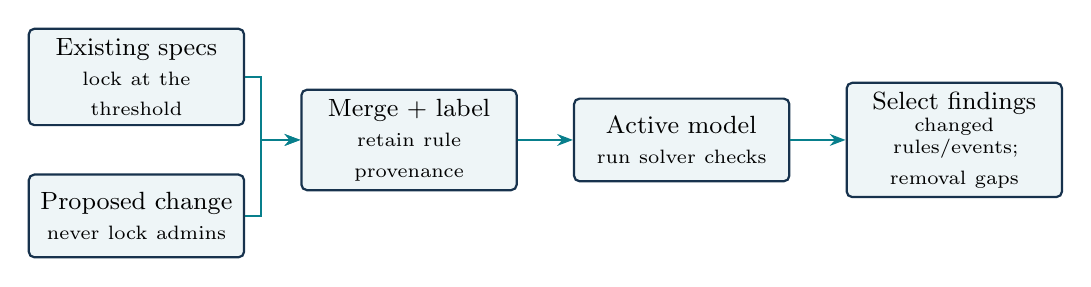
\begin{tikzpicture}[node distance=7mm,stage/.append style={text width=2.5cm}]
\node[stage] (base) {Existing specs\\\scriptsize lock at the threshold};
\node[stage,below=6mm of base] (delta) {Proposed change\\\scriptsize never lock admins};
\node[stage,right=of base,yshift=-8mm] (merge) {Merge + label\\\scriptsize retain rule provenance};
\node[stage,right=of merge] (check) {Active model\\\scriptsize run solver checks};
\node[stage,right=of check] (filter) {Select findings\\\scriptsize changed rules/events;\\removal gaps};
\draw[flow] (base.east)--++(.2,0)|-(merge.west);
\draw[flow] (delta.east)--++(.2,0)|-(merge.west);
\draw[flow] (merge)--(check);\draw[flow] (check)--(filter);
\end{tikzpicture}
}
\caption{The authentication example, checked against existing requirements.}
\end{figure}
\example{An exception that breaks an existing lockout rule}
An existing authentication specification locks accounts at a failed-login
threshold. A change adds ``administrators are never locked.'' Neither
fragment alone shows the cross-document conflict. The checker must analyze
their combined obligations while preserving which ones came from the
change.

\textbf{Input:} existing capability specifications and one OpenSpec change
directory. \textbf{Output:} a merged analysis document, the formal model
and findings, and a report focused on the change. The merge applies renamed,
removed, modified and added requirements in that order. Requirements are
matched by name; scenarios receive labels and provenance indicating existing,
added, modified or removed content. Within a modified requirement, scenario
names and normalized bodies determine those statuses. Normalization ignores
case, extra whitespace and selected Markdown marks; it does not establish
semantic equivalence. In full mode, active scenarios use R labels and removed
scenarios use X labels. In reuse mode, old labels remain fixed in the base,
new or rewritten scenarios use N labels, and superseded old scenarios are
marked replaced.
Invalid references are rejected. This produces an analysis document; it
does not archive or apply the change to the original specifications.

\begin{algorithm}[H]
\caption{Analyze a change with provenance}\label{alg:change}
\begin{algorithmic}[1]
\State Merge existing specifications with the delta and classify scenario provenance
\If{incremental mode is requested}
  \State Obtain the combined raw model by Algorithm~\ref{alg:incremental}
\Else
  \State Formalize the combined document, including removed X-labelled scenarios
\EndIf
\State Save the raw formal model before the after-change projection
\State Validate that every expected scenario label occurs exactly once
\State Identify added or modified rule IDs from labels and changed requirement text
\State Separate deleted rules as removal seeds; discard superseded old scenarios
\State Drop links and outcome-pair facts tagged with any separated/discarded rule
\State Analyze active obligations; supply usable removal seeds to the gap search
\State Select conflicts and scenarios mentioning a changed rule
\State Select ambiguities of changed rules and gaps for their reacted-to events
\State Also select gaps carrying \code{opened_by} removal attribution
\State Keep other defects in the findings artifact; present selected findings
\end{algorithmic}
\end{algorithm}

The method gives existing and changed requirements one shared vocabulary,
which makes cross-document relations visible. It is not a semantic
before/after diff: finding selection uses provenance and event relevance.
For an extracted rule without a scenario label, normalized source wording
is compared with changed or removed requirement sentences. This heuristic
can identify a separately extracted SHALL sentence; it is not verified
semantic alignment. Ordinary voted facts are retained after deletions.
Consequently, keeping removed text in the full translation can still affect
the vocabulary and assumptions even though its obligations are inactive.

The order removal illustrates the new attribution: X1 supplies the former
no-stock situation, no surviving conditional rule covers it, and
\code{opened_by: ["X1"]} makes the gap relevant to the change. The
ordinary changed-event selection also remains: a gap on an event used by
an added or modified rule is included, without claiming that the edit caused
every such gap. Existing-only findings remain saved for inspection.
\source{speccheck/change.py; speccheck/cli.py}

\subsection{Optional reuse of a saved base}\label{app:incremental}

\begin{algorithm}[H]
\caption{Translate changed scenarios against a saved base}\label{alg:incremental}
\begin{algorithmic}[1]
\Require Existing specifications $D$, delta $\Delta$, model name $m$
\State Reject multiple vocabularies, a second reader and optional text review
\State Generate labelled base text $D_b$; compute $h=\operatorname{SHA256}(D_b)$
\If{no saved base has matching text fingerprint $h$ and model name $m$}
  \State Fully formalize $D_b$ and validate all expected scenario labels
  \State Save the base model together with $h$ and $m$
\EndIf
\State Emit added or rewritten scenarios from $\Delta$ as N-labelled text $D_n$
\If{$D_n$ is empty} \State \Return the saved base model \EndIf
\State Extract new rules and symbols, retaining existing symbol definitions
\State Translate and cluster new rules in the combined vocabulary
\State Ask for domain facts only if a new symbol was added
\State Add supported facts unless implied by or inconsistent with retained assumptions
\State Restate and probe new rules; ask eligible outcome pairs involving a new rule
\State Combine new translations and assumptions with the retained base
\State \Return the raw model for projection and analysis in Algorithm~\ref{alg:change}
\end{algorithmic}
\end{algorithm}

\example{The administrator exception against a saved lockout reading.}
The base already contains the failed-attempt symbols and the lockout rule.
The exception is extracted as N1 and interpreted using that vocabulary,
possibly extending it with an administrator condition. Old definitions and
readings do not change. If extraction redeclares an old symbol name, the
old definition wins. Outcome-pair questions require at least one new rule
and retain the forty-pair cap; new facts do not trigger a complete re-probe
of the old rules. Algorithm~\ref{alg:change} then runs the normal solver checks
on the combined active model.

The saved base is accepted by generated-text fingerprint and model-name
string only. Samples, temperature, endpoint, model-weight revision, prompts
and code version are not part of that key. A mismatch rebuilds the base;
it does not switch to full formalization of the proposed change. Corrupt
cache JSON, an unusable vocabulary or failed label validation stops the run.
Supplying a saved formal model directly bypasses this cache check.

The empty-input shortcut is important. If only a requirement sentence
changes while its scenarios stay identical, $D_n$ can be empty. Adding a
requirement without scenarios can have the same result. Those sentences
are present in full mode, but this route can reuse the old model without
translating them. A separately extracted old SHALL rule is also not retired
by scenario replacement tracking alone. These are current edit-coverage
limits. Sharing symbols and rerunning solver checks does not prove that an
old interpretation remains suitable after an edit.
\source{speccheck/cli.py; speccheck/formalize.py; speccheck/probe.py; speccheck/change.py}

\clearpage
\section{A compact reference for the worked examples}\label{app:examples}

\begin{longtable}{@{}p{.17\linewidth}p{.36\linewidth}p{.41\linewidth}@{}}
\toprule
Example & Object we carry through the pipeline & What to look for \\
\midrule
\endhead
Order R2/R3 & $(s\land\neg v)\Rightarrow b$ and $\neg b$ & $s=\True,v=\False$ is a feasible trigger; no $b$ satisfies both obligations. \\
Order R1/R5 & $(s\land v)\Rightarrow f$ and $q\Rightarrow\neg f$ & $s=v=q=\True$ forces both fulfillment and non-fulfillment. Real-world feasibility is a separate question. \\
Order quiet gap & No conditional antecedent holds & $s=c=q=\False$ leaves R3 active as a prohibition, but no conditional rule reacts. Waiting may be intended. \\
Order removal & Old R2 is retained separately as X1 & With R1 still active, $s=\True,v=c=q=\False$ is uncovered and attributed to X1. This is a constructed change. \\
Order scenario & $\Phi\land\neg(s\land v)\land f$ & $s=c=q=b=\False,f=\True$ is allowed by the encoded rules. R1 did not say ``only if.'' \\
Authentication & $(n=5)\Rightarrow\ell$ versus $(n\ge5)\Rightarrow\ell$ & At $n=6,\ell=\False$, the first holds and the second fails. This witness is an illustration of the semantic distinction. \\
Deletion D2/D4 & Confirmation $d$, removal $m$, retention $k$ & $d\Rightarrow m$ and $k$ coexist unless an assumed relation connects $m$ to $\neg k$. The relation must be shown to the reviewer. \\
\bottomrule
\end{longtable}

The short letters make the formulas easier to read. The deletion example shows only the outcomes needed here; D4 also describes hiding the record. Sample splits such as $[5,3]$ are made-up examples of the algorithm, not measured model responses.

\section{Saved results and offline replay}\label{app:artifacts}

\begin{table}[H]
\centering
\begin{tabularx}{\linewidth}{@{}lX@{}}
\toprule
Output & Contents and use \\
\midrule
\code{formal.json} & Typed symbols, translated rules, assumed facts, statuses, alternatives and probe evidence. Saved before removed/replaced rules are separated in change mode. Additional vocabularies use numbered files. \\
\code{findings.json} & Finding types, rule IDs, witnesses and any assumptions, doubt markers or support counts. Generated explanations may be included. \\
Review report & The findings and their evidence, with explanations when an LLM is used. \\
Merged specification & Full change mode saves the combined text, including removed scenarios, with labels and provenance. \\
Incremental input & Only the added or rewritten scenario text, alongside the saved base model used for translation. \\
Text suggestions & Proposed rewrites from the optional text review. \\
\bottomrule
\end{tabularx}
\caption{What the checker saves and how each output is used.}
\end{table}

The solver checks can be rerun from a saved formal model without a model server. Use a separate output directory to preserve the original results. Without a model-server URL, the CLI writes the solver evidence and leaves out explanatory prose and scenarios selected by the LLM judge. The supplied formal model stays in its original location.

For change replay, retain the original base specifications, change directory and execution mode as well as the raw formal model. The CLI saves \code{formal.json} before it removes deleted or replaced rules. Replaying that file as an ordinary specification would treat those rules as active and can change the result. The change route must reconstruct provenance, validate labels and apply the after-change projection first. Its separate removed-rule collection supplies gap seeds; replaced old scenarios do not.

Full change runs save \code{merged.md}; incremental runs save \code{new.md}. The reusable base is stored in \code{openspec/.speccheck/base.json}. A supplied \code{--formal} file bypasses cache creation and validation, so the person replaying it must ensure the base, delta and labels match. These filenames describe the saved artifacts; they are not additional evaluation evidence.

Our abbreviations follow the archived order model. The older test fixture uses different names. Compare rule sets and formulas; witnesses can differ for the same finding.

\clearpage
\section{Follow one saved requirement through the files}\label{app:walkthrough}

These are the requirement text and selected fields from the saved order example. Some fields are omitted for space; the values shown are unchanged.

\textbf{1. The source requirements.} The input carries the IDs that must survive extraction.
\begin{lstlisting}
- R2: WHEN an order is submitted AND inventory is unavailable, THE Order System SHALL place the order on backorder.
- R3: THE Order System SHALL NOT place any order on backorder.
\end{lstlisting}
\source{specs/order/requirements.md}

\textbf{2. One symbol.} The event marker is metadata used by the checks. It is not a temporal transition operator.
\begin{lstlisting}
{
  "name": "order_submitted",
  "sort": "Bool",
  "event": true
}
\end{lstlisting}

\textbf{3. The selected R2 translation.} The two formula fields become an implication. The retained status describes the pipeline's selected reading; it is not proof of faithful translation.
\begin{lstlisting}
{
  "id": "R2",
  "status": "accepted",
  "clusters": [8],
  "entropy": 0.0,
  "antecedent": "(and order_submitted (not inventory_available))",
  "consequent": "order_on_backorder"
}
\end{lstlisting}
\source{specs/order/formal.json}

Read this as: if submission occurs and stock is unavailable, backordering is required. In the paper's shorter notation it is $(s\land\neg v)\Rightarrow b$. R3's consequent is \code{(not order_on_backorder)}, with antecedent \code{true}. Sharing the exact same outcome symbol is what makes the collision visible.

\clearpage
\textbf{4. The solver trace, written as explanatory pseudocode.} This trace illustrates the checks; it is not a literal saved API log.
\begin{lstlisting}
T := order_submitted AND NOT inventory_available
check(T)                         -> SAT
check(T AND all_rule_implications)-> UNSAT
delete unnecessary core members  -> R2, R3
find a witness for T              -> submitted=true, stock=false
\end{lstlisting}

Removing either R2 or R3 makes this two-rule explanation satisfiable in the triggering situation. That is the local explanation we need. It does not claim that every possible conflict in the whole document has been enumerated.

\textbf{5. The saved finding.} These selected fields retain the evidence independently of generated prose.
\begin{lstlisting}
{
  "type": "conflict",
  "rules": ["R2", "R3"],
  "when": {
    "inventory_available": false,
    "order_submitted": true
  }
}
\end{lstlisting}
\source{specs/order/findings.json}

\textbf{6. The question for the author.} We could put it this way: ``An order arrives without stock. R2 says to backorder it; R3 forbids that. Should we allow backorders, or revise the no-stock response?'' The requirements author chooses the policy.

The same discipline applies to an assumption-dependent conflict: show the assumed relation as well as the rules. For the shortened deletion example, the reviewer needs to see $(d\land m)\Rightarrow\neg k$, because whether removal excludes retention is precisely the disputed meaning.

\textbf{Checking the examples.} The 40 offline checks cover the authentication findings, the saved order model, the example formulas and sample splits, gap sensitivity, removal attribution and retirement, a saved removal finding, and the two scenario-only input limitations. They check the logic and input selection without a model server. The experimental results discussed earlier come from the original saved runs.

\end{document}
